\documentclass[letterpaper, 12pt]{article}

% \usepackage[showframe, margin=1in, top=0.25in, bottom=0.25in, includeheadfoot, headheight=0.5in]{geometry}
\usepackage[margin=1in, top=0.25in, bottom=0.25in, includeheadfoot, headheight=0.5in]{geometry}

\AddToHook{cmd/section/before}{\clearpage}

\usepackage[table]{xcolor}
\colorlet{listingback}{gray!20}
\definecolor{headingcolor}{RGB}{110,34,54}

\usepackage{fancyhdr}
\renewcommand{\sectionmark}[1]{\markboth{#1}{#1}}

% Used to detect whether a section is an appendix to print the right thing in the footer
\usepackage{etoolbox}
\newtoggle{inappendix}
\pretocmd{\appendix}{\clearpage\toggletrue{inappendix}}{}{}

% Save standard definitions for head and foot rules (lines separating header and footer from text)
\let\HeadRule\headrule
\let\FootRule\footrule
% Add color to the standard definitions
\renewcommand{\headrule}{\color{headingcolor}\HeadRule}
\renewcommand{\footrule}{\textcolor{headingcolor}{\FootRule}}

% IMPORTANT: This command should not be called directly. Use \preamble.
% Macro to insert the title page for each lab.
% The argument is the title of the lab.
\newcommand{\inserttitlepage}[1]
{
    \begin{titlepage}
    \centering
    
\includegraphics[scale=0.5]{images/nexus_lab_logo.png}

    \vspace*{\baselineskip}

    \textbf{\Large OpenStack Labs}

    \vspace*{\baselineskip}

    \textbf{\Large #1}
    \vspace*{\fill}
\end{titlepage}
}

% IMPORTANT: This command should not be called directly. Use \preamble.
% Macro to define header and footer for each lab.
% The argument is the title of the lab.
\newcommand{\headfoot}[1]
{
    \fancypagestyle{fancy}
    {
        \fancyhf{}
        \fancyhead[L]{\footnotesize #1}
        \fancyhead[R]{
\includegraphics[height=0.85\headheight]{images/nexus_lab_logo.png}}
        \fancyfoot[L]{%
            \footnotesize%
            \ifnum\value{section}>0%
            \iftoggle{inappendix}{Appendix \thesection: \rightmark}{Section \thesection: \rightmark}%
            \fi}
        \fancyfoot[R]{\footnotesize\thepage}
        \renewcommand{\headrulewidth}{1.5pt}
        \renewcommand{\footrulewidth}{1.5pt}
    }
}

% Macro to insert title page, define header and footer, and insert table of contents and about section for each lab.
% The argument is the title of the lab.
\newcommand{\preamble}[1]
{
    \pagenumbering{roman}
    \inserttitlepage{#1}
    \headfoot{#1}

    % Insert table of contents
    \pagestyle{fancy}
    \tableofcontents
    \clearpage

    \section*{About This Document}
    \label{sec:about_this_document}
    \begin{itemize}
        \item This document was developed by a team at the University of Tennessee at Chattanooga led by Dr. Mengjun Xie
        (\href{mailto:mengjun-xie@utc.edu}{\textbf{mengjun-xie@utc.edu}}).
        \item The development of this document was supported by a National Centers of Academic Excellence in Cybersecurity Grant (\#H98230-20-1-0351), housed at the National Security Agency.
        \item This document is licensed with a Creative Commons Attribution 4.0 International License.
    \end{itemize}
    \clearpage
}

% Macro to insert the Lab Settings page for each lab. Call after the Introduction and Objectives sections.
\newcommand{\labsettings}
{
    \section*{Lab Settings}
    \label{sec:lab_settings}
    \addcontentsline{toc}{section}{\nameref{sec:lab_settings}}
    The information in the table below will be needed in order to complete the lab.
    The task sections below provide details on the use of this information.
    \begin{table*}[htbp]
        \centering
        \begin{tabular}{|c|c|c|c|}
            \hline
            \rowcolor{gray!20} \textbf{Virtual Machine} & \textbf{IP Address} & \textbf{Account} & \textbf{Password} \\
            \hline
            \multirow{2}{*}{\texttt{workstation}} & \multirow[t]{2}{*}{\texttt{ens3: 192.168.1.21}}  & \multirow{2}{*}{\texttt{ubuntu}} & \multirow{2}{*}{\texttt{ubuntu}} \\
                                                  & \multirow[t]{2}{*}{\texttt{ens4: 172.25.250.21}} &                                  &                                  \\
            \hline
            \multirow{2}{*}{\texttt{devstack}}    & \multirow[t]{2}{*}{\texttt{ens3: 192.168.20}}    & \multirow{2}{*}{\texttt{ubuntu}} & \multirow{2}{*}{\texttt{ubuntu}} \\
                                                  & \multirow[t]{2}{*}{\texttt{ens4: 172.25.250.20}} &                                  &                                  \\
            \hline
        \end{tabular}
    \end{table*}
    \clearpage

    % IMPORTANT(lucas): If another frontmatter section ever gets placed after this, this command needs to be moved
    % to the end of that section.
    % I have placed this here and not in each lab purely for convenience and to ensure I don't forget any.
    \pagenumbering{arabic}
}

% Sans-serif font
\renewcommand{\familydefault}{\sfdefault}
\newcommand{\texttildemid}{{\raisebox{0.5ex}{\texttildelow}}}

\usepackage{enumitem}
\renewcommand{\labelenumi}{\textbf{\thesection.\arabic{enumi}.}}

% Try to forbid widows and orphans
\widowpenalty10000
\clubpenalty10000

\usepackage{graphicx}
\usepackage{hyperref}
\hypersetup{colorlinks=true,linkcolor=black,urlcolor={[named] headingcolor}}

\usepackage{sectsty}
\sectionfont{\color{headingcolor}}

% Table of Contents
\usepackage{bookmark}
\usepackage[titles]{tocloft}
\usepackage[title]{appendix}
\renewcommand{\cfttoctitlefont}{\Large\bfseries\color{headingcolor}}
\renewcommand{\cftsecfont}{\normalfont\normalsize}
\renewcommand{\cftsecpagefont}{\normalfont\normalsize}
\renewcommand{\cftdotsep}{0} % Make dots small and close together
\renewcommand{\cftsecleader}{\cftdotfill{\cftdotsep}} % Add dots after section titles
% Make dots go all the way to the page number
\renewcommand{\cftsecfillnum}[1]{{\cftsecleader}\nobreak{\cftsecpagefont #1}\cftsecafterpnum\par}

\usepackage{multirow}
\setlength{\tabcolsep}{16pt}
\renewcommand{\arraystretch}{1.1}

% For nice-looking boxes
\usepackage[most]{tcolorbox}
\usepackage{listings}
\usepackage{lstautogobble}
\lstset{
  frame=none,
  language=Bash,
  showstringspaces=false,
  basicstyle={\linespread{1.1}\footnotesize\ttfamily\selectfont},
  numbers=none,
  breaklines=true,
  breakatwhitespace=true,
  tabsize=3,
  columns=fullflexible,
  keepspaces=true,
  escapeinside={(*@}{@*)},
  literate={~}{{\texttildemid}}{1}
           {\#}{\#}{1},
  autogobble=true
}

\tcolorboxenvironment{lstlisting}
{
    spartan,
    colframe=gray!50,
    boxsep=0mm,
    left=1mm,
    right=1mm,
    top=-1mm,
    bottom=-1mm,
    colback=gray!20
}

% Hacky solution for now, would like to have just one environment and make several tcolorboxes by passing different
% colors as parameters, but that is giving errors
\makeatletter
\tcbset{
  note/.style={%
        enhanced,
        breakable,
        colback=blue!10!white,
        colframe=blue!80!white,
        attach boxed title to top left={yshift*=-\tcboxedtitleheight},
        title={#1},
        boxed title size=title,
        boxed title style={%
            sharp corners,
            rounded corners=northwest,
            colback=tcbcolframe,
            boxrule=0pt,
        },
        underlay boxed title={%
            \path[fill=tcbcolframe] (title.south west)--(title.south east)
                to[out=0, in=180] ([xshift=5mm]title.east)--
                (title.center-|frame.east)
                [rounded corners=\kvtcb@arc] |-
                (frame.north) -| cycle;
        },
    }
}
\makeatother

\makeatletter
\tcbset{
    stop/.style={%
        enhanced,
        breakable,
        colback=white,
        colback=red!10!white,
        colframe=red!80!white,
        attach boxed title to top left={yshift*=-\tcboxedtitleheight},
        title={#1},
        boxed title size=title,
        boxed title style={%
            sharp corners,
            rounded corners=northwest,
            colback=tcbcolframe,
            boxrule=0pt,
        },
        underlay boxed title={%
            \path[fill=tcbcolframe] (title.south west)--(title.south east)
                to[out=0, in=180] ([xshift=5mm]title.east)--
                (title.center-|frame.east)
                [rounded corners=\kvtcb@arc] |-
                (frame.north) -| cycle;
        },
    }
}
\makeatother

\makeatletter
\tcbset{
    tip/.style={%
        enhanced,
        breakable,
        colback=white,
        colback=green!10,
        colframe=green!70!black,
        attach boxed title to top left={yshift*=-\tcboxedtitleheight},
        fonttitle=\bfseries,
        title={#1},
        boxed title size=title,
        boxed title style={%
            sharp corners,
            rounded corners=northwest,
            colback=tcbcolframe,
            boxrule=0pt,
        },
        underlay boxed title={%
            \path[fill=tcbcolframe] (title.south west)--(title.south east)
                to[out=0, in=180] ([xshift=5mm]title.east)--
                (title.center-|frame.east)
                [rounded corners=\kvtcb@arc] |-
                (frame.north) -| cycle;
        },
    }
}
\makeatother

% The commands below define environments for colored boxes. They are used like
% \begin{notebox}
% ...
% \end{notebox}
\newtcolorbox{notebox}{note={Note}}
\newtcolorbox{stopbox}{stop={Stop}}
\newtcolorbox{tipbox}{tip={Tip}}


\begin{document}
\begin{titlepage}
    \centering
    
\includegraphics[scale=0.5]{images/nexus_lab_logo.png}

    \vspace*{\baselineskip}

    \textbf{\Large OpenStack Labs}

    \vspace*{\baselineskip}

    \textbf{\Large Lab 08: Deploying an External Instance}
    \vspace*{\fill}
\end{titlepage}

\fancypagestyle{fancy}
{
    \fancyhf{}
    \fancyhead[L]{\footnotesize Lab 08: Deploying an External Instance}
    \fancyhead[R]{
\includegraphics[height=0.85\headheight]{images/nexus_lab_logo.png}}
    \fancyfoot[R]{\footnotesize\thepage}
    \renewcommand{\headrulewidth}{0pt}
}

\pagestyle{fancy}
\tableofcontents
\clearpage

\section*{Introduction}
\label{sec:introduction}
\addcontentsline{toc}{section}{\nameref{sec:introduction}}
In this lab, you will manage external networks, floating IP addresses, implement security, and launch an external
instance.

\section*{Objectives}
\label{sec:objectives}
\addcontentsline{toc}{section}{\nameref{sec:objectives}}
\begin{itemize}[itemsep=0pt]
    \item Manage external networks.
    \item Manage OpenStack routers.
    \item Manage floating IP addresses.
    \item Manage SSH key pairs and security groups.
    \item Launch and verify an external instance.
\end{itemize}
\clearpage

\section*{Lab Settings}
\label{sec:lab_settings}
\addcontentsline{toc}{section}{\nameref{sec:lab_settings}}
The information in the table below will be needed in order to complete the lab. The task sections below provide details
on the use of this information.
\begin{table*}[htbp]
\centering
\begin{tabular}{|c|c|c|c|}
    \hline
    \rowcolor{gray!20} \textbf{Virtual Machine} & \textbf{IP Address} & \textbf{Account} & \textbf{Password} \\
    \hline
    \multirow{2}{*}{\texttt{workstation}} & \multirow[t]{2}{*}{\texttt{ens3: 192.168.1.20}}  & \multirow{2}{*}{\texttt{ubuntu}} & \multirow{2}{*}{\texttt{ubuntu}} \\
                                          & \multirow[t]{2}{*}{\texttt{ens4: 172.25.250.20}} &                                  &                                  \\
    \hline
    \multirow{2}{*}{\texttt{devstack}}    & \multirow[t]{2}{*}{\texttt{ens3: 192.168.1.21}}  & \multirow{2}{*}{\texttt{ubuntu}} & \multirow{2}{*}{\texttt{ubuntu}} \\
                                          & \multirow[t]{2}{*}{\texttt{ens4: 172.25.250.21}} &                                  &                                  \\
    \hline
\end{tabular}
\end{table*}
\clearpage

\section{Managing External Networks}
\label{sec:managing_external_networks}
In this task, you will use the \textit{Horizon Dashboard} and the \textbf{OpenStack Unified CLI} to create and configure
an external network.

\begin{enumerate}
    \item Open the web browser. Navigate to \textbf{192.168.1.20} and log in to the dashboard as \textbf{admin}
    with the password \textbf{secret}.

    \item Switch to the \textbf{demo} project. Navigate to \textbf{Admin $>$ Network $>$ Routers}. Check the box in the
    same row as \textbf{router1}, then click \textbf{Delete Routers}.

    \begin{center}
        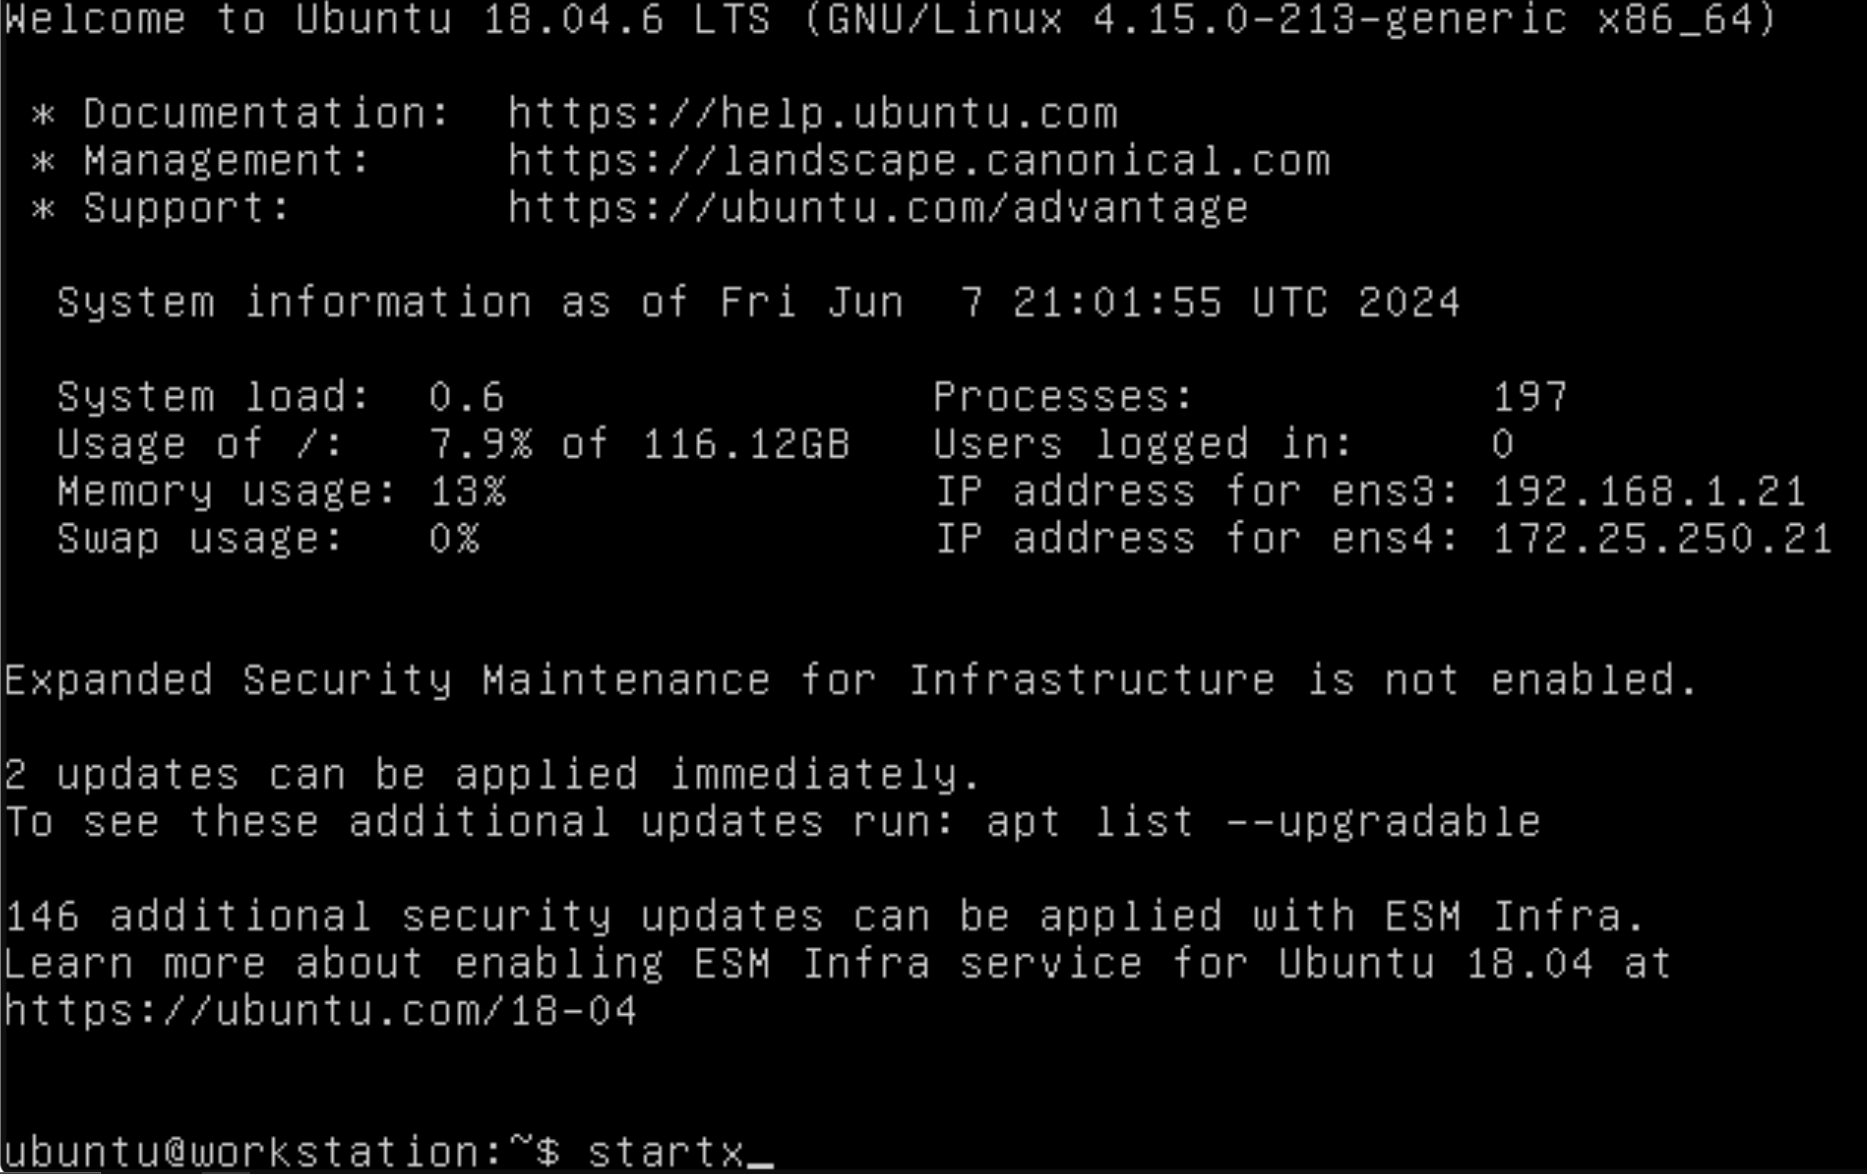
\includegraphics[width=\linewidth]{images/part1/step2.png}
    \end{center}

    \item Now, navigate to \textbf{Networks}. Check the box in the same row as \textbf{public}, then click
    \textbf{Delete Networks}.

    \begin{center}
        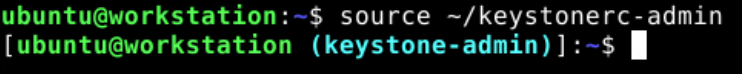
\includegraphics[width=\linewidth]{images/part1/step3.png}
    \end{center}

    \item Click \textbf{Create Network}.
    
    \begin{center}
        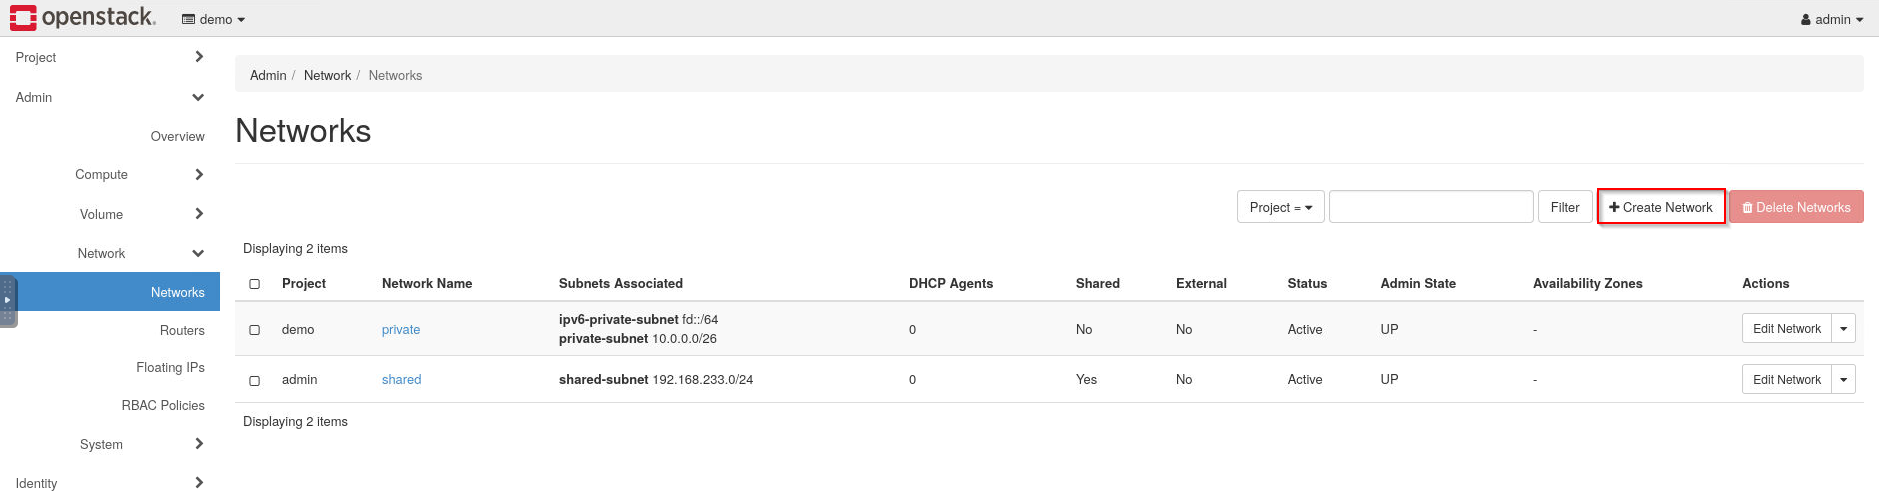
\includegraphics[width=\linewidth]{images/part1/step4.png}
    \end{center}
    
    \item Enter \textbf{net1} in the \textit{Network Name} field. Select \textbf{demo} in the \textit{Project} dropdown.
    For \textit{Provider Network Type}, select \textbf{Flat}. Enter \textbf{public} into the \textit{Physical Network}
    field. Check the \textit{Shared} and \textit{External Network} check boxes, and ensure the \textit{Create Subnet}
    check box is checked. Click \textbf{Next} to go to the \textit{Subnet} tab.

    \begin{center}
        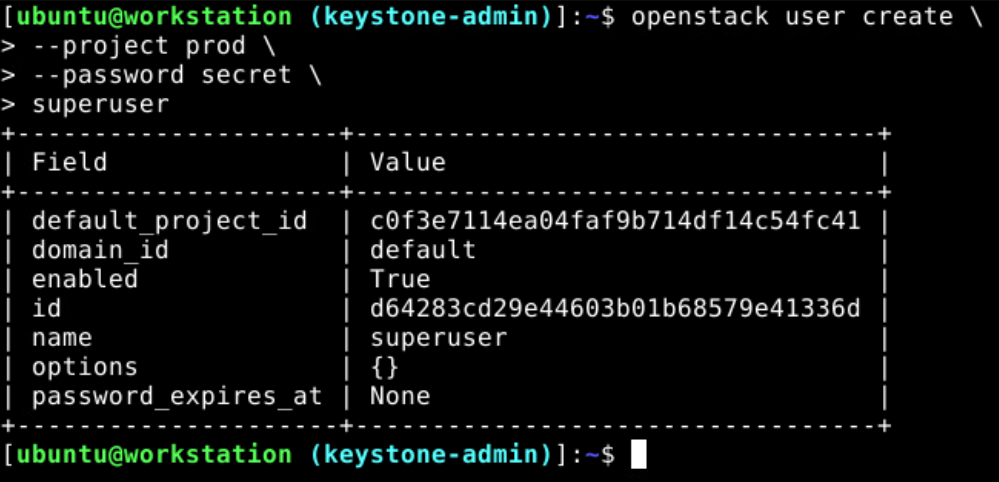
\includegraphics[width=\linewidth]{images/part1/step5.png}
    \end{center}

    \item In the \textit{Subnet} tab, enter \textbf{subnet1} in the \textit{Subnet Name} field, and enter
    \textbf{172.25.250.0/24} in the \textit{Network Address} field. Click \textbf{Next} to go to the \textit{Subnet
    Details} tab.

    \begin{center}
        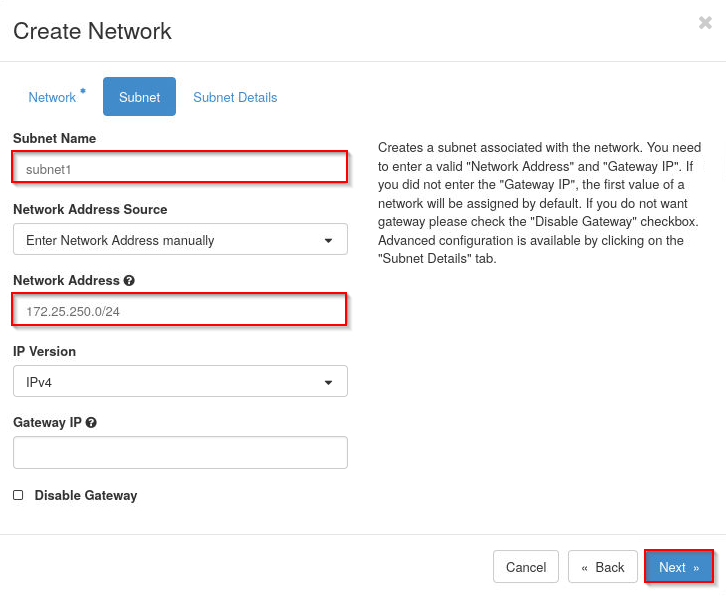
\includegraphics[width=\linewidth]{images/part1/step6.png}
    \end{center}

    \item In the \textit{Subnet Details} tab, uncheck the \textit{Enable DHCP} check box. Enter
    \textbf{172.25.250.5, 172.25.250.100} in the \textit{Allocation Pools} field. Click \textbf{Create} to create the
    network and subnet.

    \begin{center}
        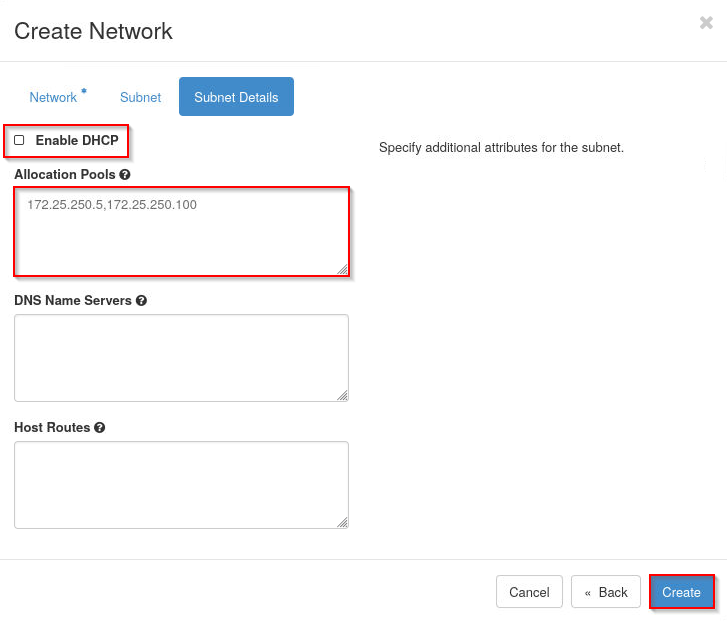
\includegraphics[width=\linewidth]{images/part1/step7.png}
    \end{center}

    \item Log out of the \textit{Horizon Dashboard} and close the web browser.
    
    \item Open a terminal window and source the keystone credentials for the \textbf{admin} user.
\begin{lstlisting}
ubuntu@workstation:~$ source ~/keystonerc-admin
\end{lstlisting}

    \begin{center}
        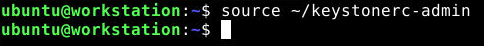
\includegraphics[width=\linewidth]{images/part1/step9.png}
    \end{center}

    \item Delete the \textbf{subnet1} subnet.
\begin{lstlisting}
ubuntu@workstation:~$ openstack subnet delete subnet1
\end{lstlisting}

    \begin{center}
        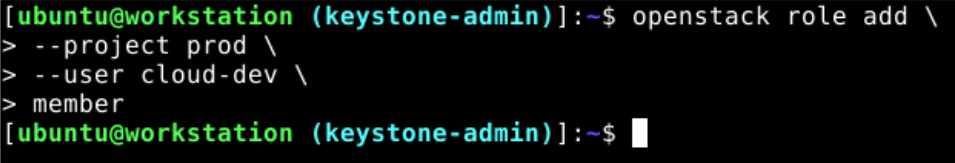
\includegraphics[width=\linewidth]{images/part1/step10.png}
    \end{center}

    \item Delete the \textbf{net1} network.
\begin{lstlisting}
ubuntu@workstation:~$ openstack network delete net1
\end{lstlisting}

    \begin{center}
        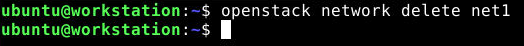
\includegraphics[width=\linewidth]{images/part1/step11.png}
    \end{center}

    \item Create an external network named \textbf{external}. Set the network type to \textbf{flat} and the physical
    network to \textbf{public}. Set the network as shared and external.
\begin{lstlisting}
ubuntu@workstation:~$ openstack network create external \
> --external --share \
> --provider-network-type flat \
> --provider-physical-network public
\end{lstlisting}

    \begin{center}
        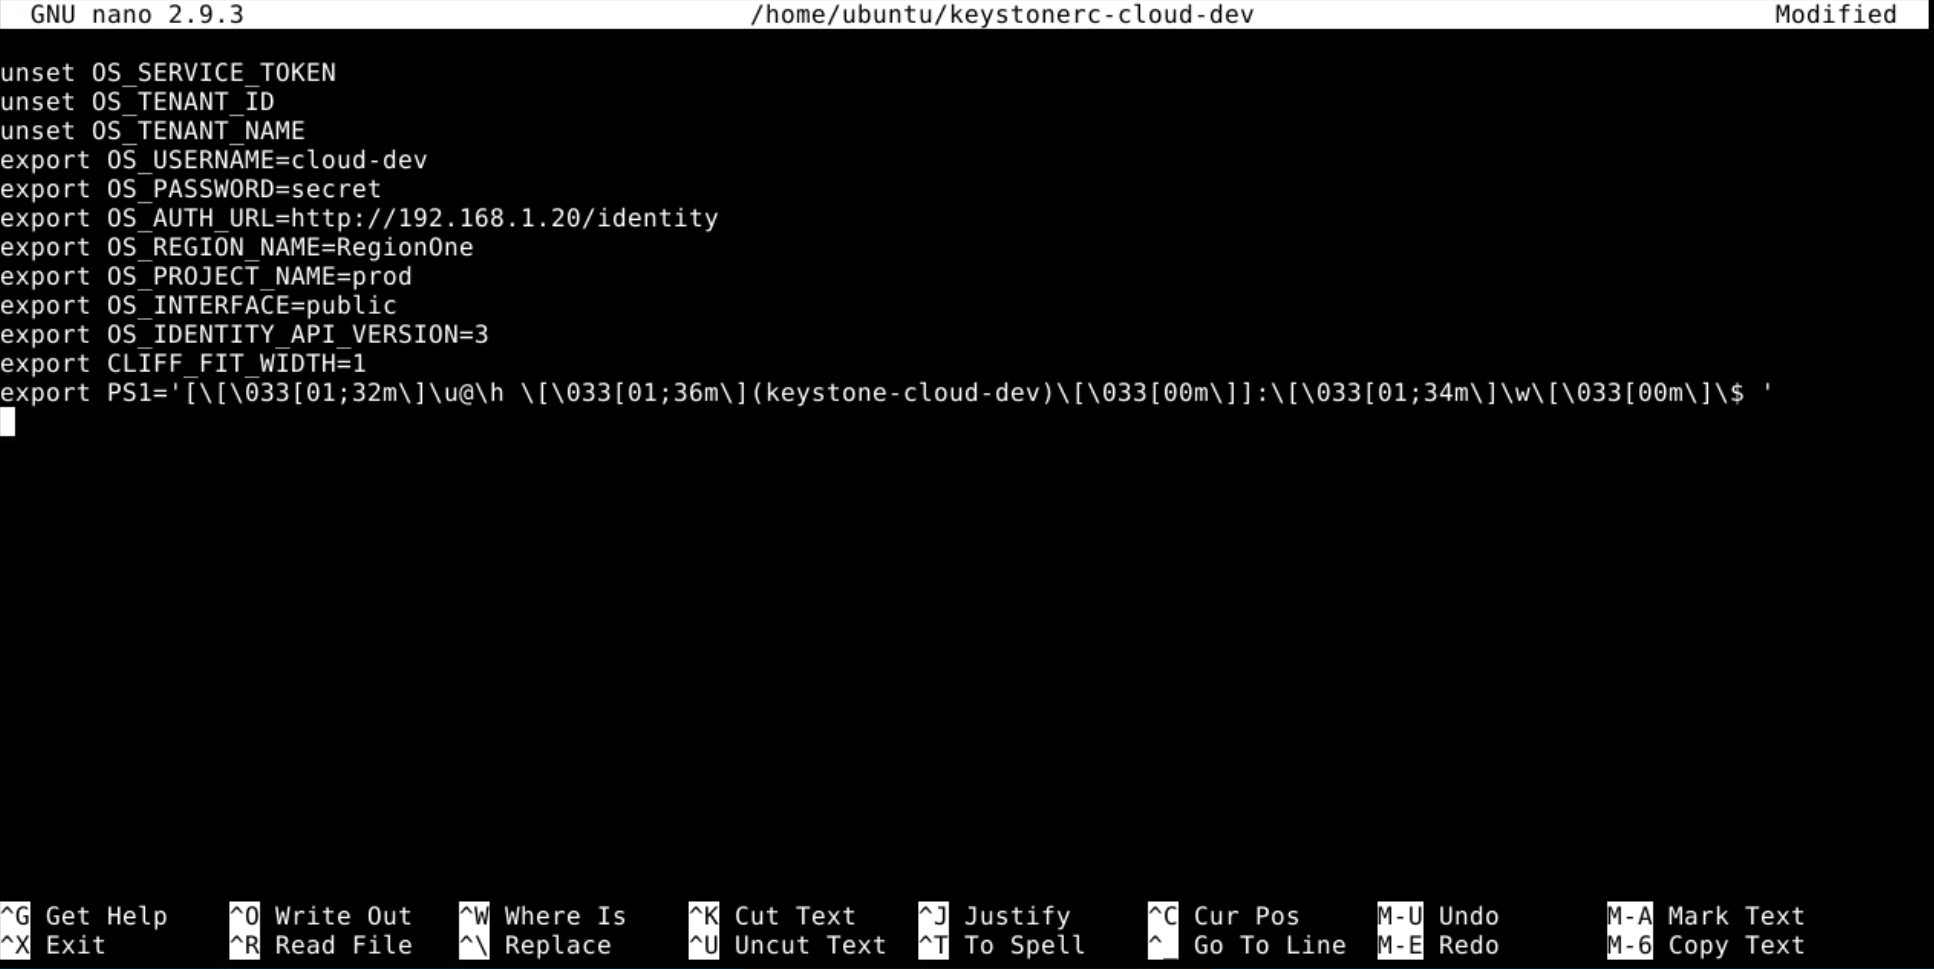
\includegraphics[width=\linewidth]{images/part1/step12.png}
    \end{center}

    \begin{tipbox}{}
        WHen typing the command, make sure there is a space between \texttt{external} and the \texttt{\textbackslash}
        character, and press \textbf{Enter} to get the \texttt{>} and continue typing the rest of the command.
    \end{tipbox}

    \item Create a subnet named \textbf{subext} in the \textbf{external} network. Give the subnet a range of
    \textbf{172.25.250.60} to \textbf{172.25.250.80}. Disable DHCP services for the subnet and use the address
    \textbf{172.25.250.254} as the gateway as well as the DNS name server.
\begin{lstlisting}
ubuntu@workstation:~$ openstack subnet create \
> --subnet-range 172.25.250.0/24 \
> --no-dhcp \
> --gateway 172.25.250.254 \
> --dns-nameserver 172.25.250.254 \
> --allocation-pool start=172.25.250.60,end=172.25.250.80 \
> --network external \
> subext
\end{lstlisting}

    \begin{center}
        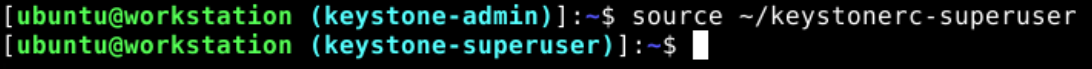
\includegraphics[width=\linewidth]{images/part1/step13.png}
    \end{center}

    \item Leave the terminal window open and continue to the next task.

\end{enumerate}

\section{Preparing OpenStack Routers to Deploy an Instance}
\label{sec:preparing_openstack_routers_to_deploy_an_instance}
In this task, you will create and configure a router using the \textit{Horizon Dashboard} and \textit{OpenStack Unified
CLI} and use command line tools to test the connectivity of the router.

\begin{enumerate}
    \item Open the web browser and navigate to \textbf{192.168.1.20}. Log into the dashboard as \textbf{admin} with the
    password \textbf{secret}.

    \item Switch to the \textbf{demo} project and navigate to \textbf{Project $>$ Network $>$ Routers}. Click
    \textbf{Create Router} to create a new router.
    
    \begin{center}
        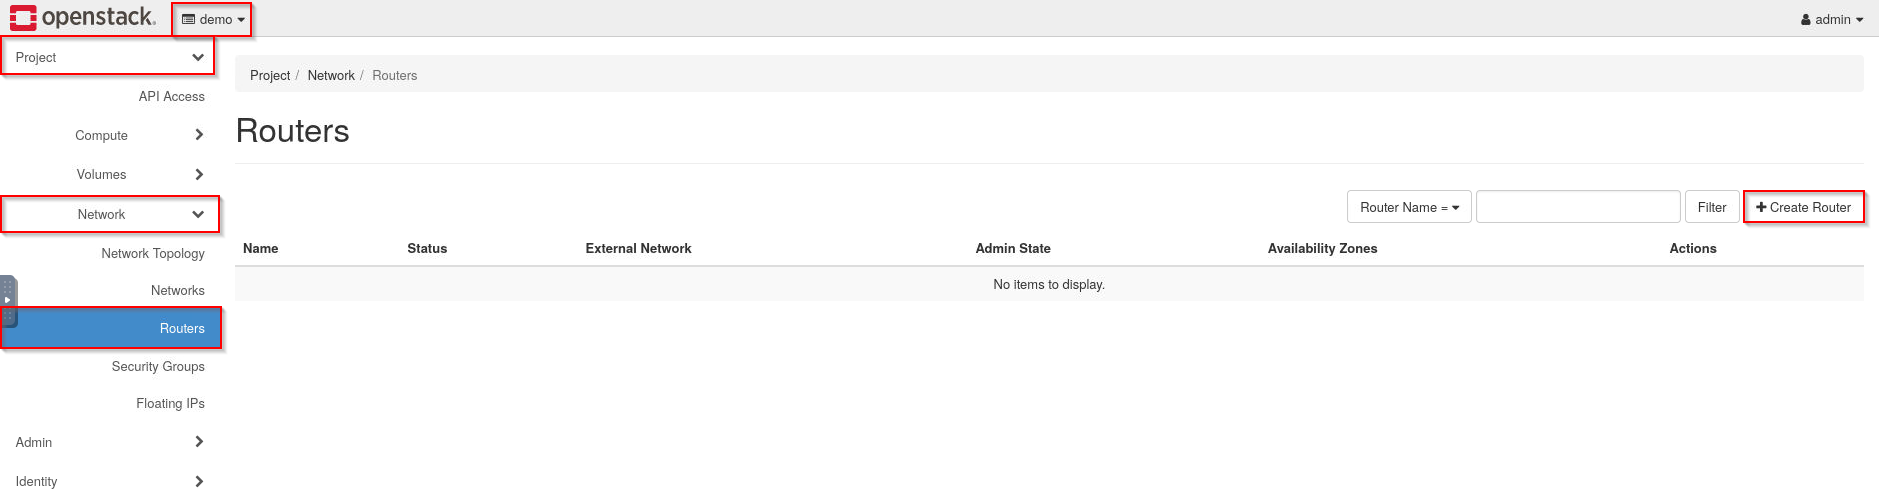
\includegraphics[width=\linewidth]{images/part2/step2.png}
    \end{center}

    \item Enter \textbf{router1} in the \textit{Router Name} field and select \textbf{external} in the \textit{External
    Network} dropdown. Click \textbf{Create Router}.

    \begin{center}
        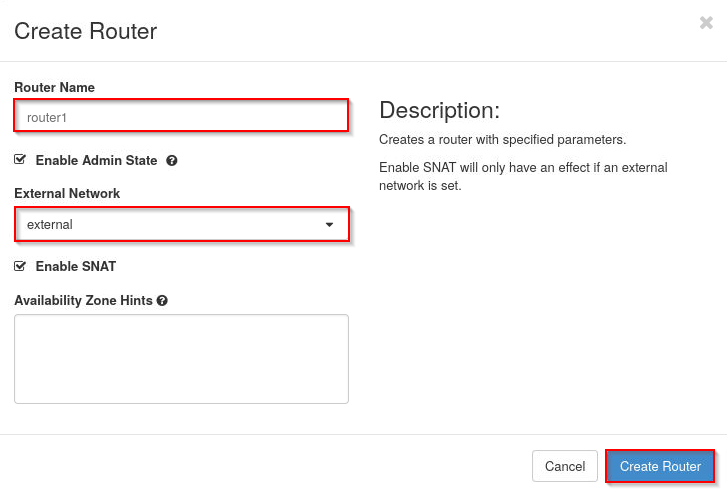
\includegraphics[width=\linewidth]{images/part2/step3.png}
    \end{center}

    \item Click the router name, \textbf{router1}, to access its details.
    
    \begin{center}
        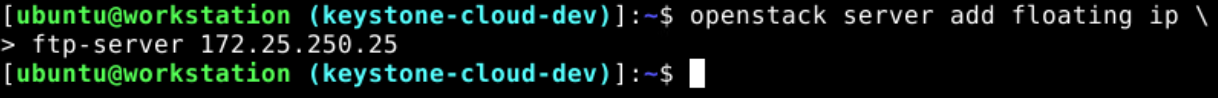
\includegraphics[width=\linewidth]{images/part2/step4.png}
    \end{center}

    \item Click the \textbf{Interfaces} tab to manage the interfaces for the router. Click \textbf{Add Interface} to add
    a new interface.

    \begin{center}
        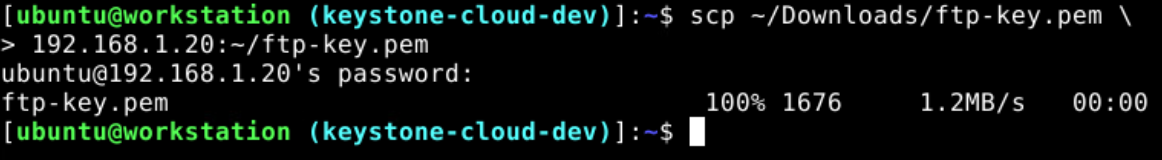
\includegraphics[width=\linewidth]{images/part2/step5.png}
    \end{center}

    \item Select \textbf{shared: 172.25.233.0/24 (shared-subnet)} from the \textit{Subnet} dropdown and click
    \textbf{Submit} to add the interface.

    \begin{center}
        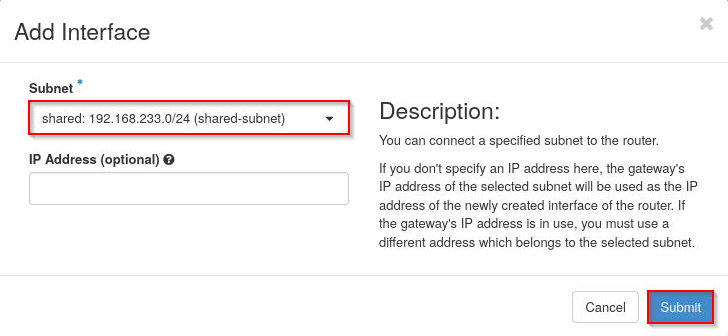
\includegraphics[width=\linewidth]{images/part2/step6.png}
    \end{center}

    \item Log out of the dashboard and close the web browser.
    
    \item Open a terminal window if one is not already open, and source the \textbf{admin} credentials.
\begin{lstlisting}
ubuntu@workstation:~$ source ~/keystonerc-admin
\end{lstlisting}

    \begin{center}
        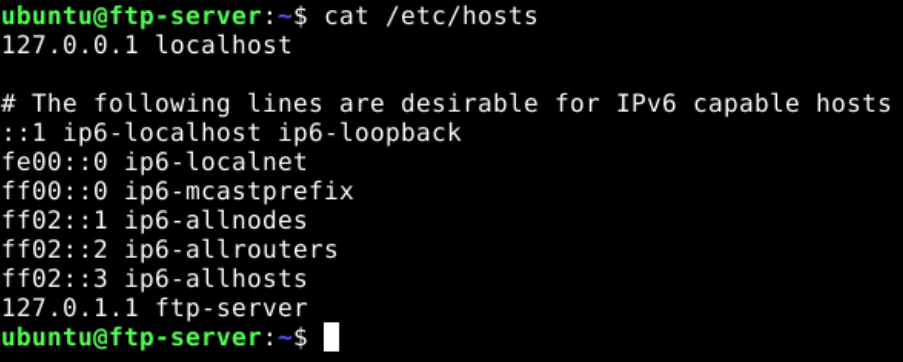
\includegraphics[width=\linewidth]{images/part2/step8.png}
    \end{center}

    \item Show the details of \textbf{router1}. Copy the \texttt{subnet\_id} from the
    \texttt{interfaces\_info} row of the output.
\begin{lstlisting}
ubuntu@workstation:~$ openstack router show router1
\end{lstlisting}

    \begin{center}
        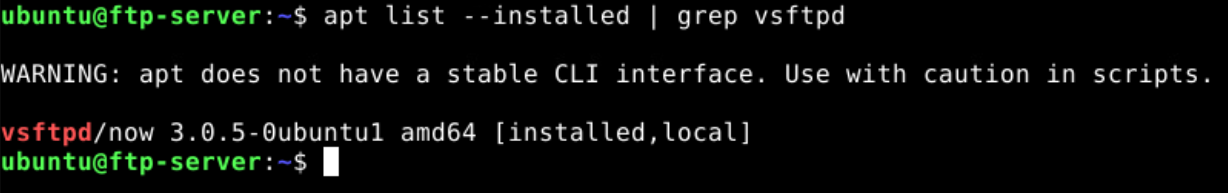
\includegraphics[width=\linewidth]{images/part2/step9.png}
    \end{center}

    \begin{tipbox}{}
        You can copy from the terminal to the clipboard the keyboard shortcut \textbf{Ctrl+Shift+C}.
    \end{tipbox}

    \item Delete the interface in the \textbf{shared} subnet for the \textbf{router1} router using the command below.
    Substitute the subnet ID with the one you copied previously. Make sure not to include any characters besides numbers
    and hyphens.
\begin{lstlisting}
ubuntu@workstation:~$ openstack router remove subnet router1 \
> 85998680-f76d-4cba-887c-f4946a26e071
\end{lstlisting}

    \begin{center}
        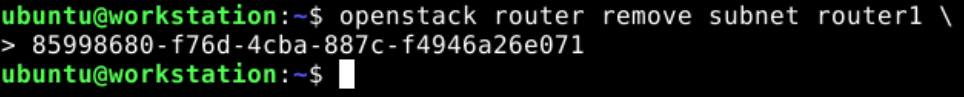
\includegraphics[width=\linewidth]{images/part2/step10.png}
    \end{center}

    \begin{tipbox}{}
        You can paste from the clipboard into the terminal with the keyboard shortcut \textbf{Ctrl+Shift+V}.
    \end{tipbox}

    \item Unset the \textbf{external} network as the gateway for the router.
\begin{lstlisting}
ubuntu@workstation:~$ openstack router unset --external-gateway router1
\end{lstlisting}

    \begin{center}
        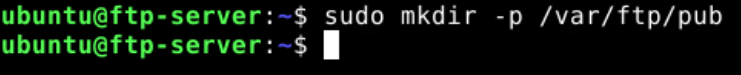
\includegraphics[width=\linewidth]{images/part2/step11.png}
    \end{center}

    \item Delete the \textbf{router1} router.
\begin{lstlisting}
ubuntu@workstation:~$ openstack router delete router1
\end{lstlisting}

    \begin{center}
        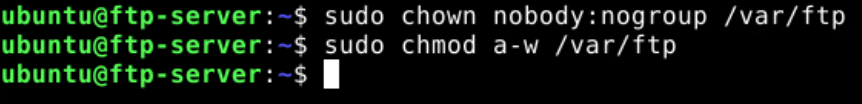
\includegraphics[width=\linewidth]{images/part2/step12.png}
    \end{center}

    \item Create a router named \textbf{exercise-router}.
\begin{lstlisting}
ubuntu@workstation:~$ openstack router create exercise-router
\end{lstlisting}

    \begin{center}
        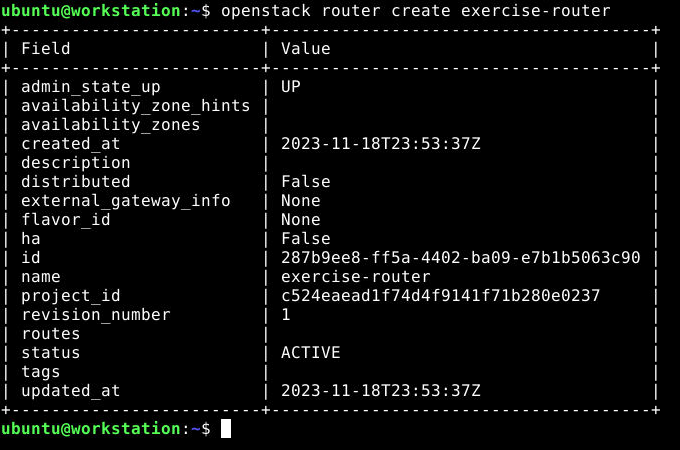
\includegraphics[width=\linewidth]{images/part2/step13.png}
    \end{center}

    \item Connect the router to the \textbf{shared-subnet} subnet.
\begin{lstlisting}
ubuntu@workstation:~$ openstack router add subnet \
> exercise-router shared-subnet
\end{lstlisting}

    \begin{center}
        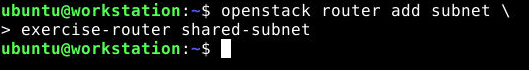
\includegraphics[width=\linewidth]{images/part2/step14.png}
    \end{center}

    \item Set the \textbf{external} network as the gateway for the router.
\begin{lstlisting}
ubuntu@workstation:~$ openstack router set \
> --external-gateway external \
> exercise-router
\end{lstlisting}

    \begin{center}
        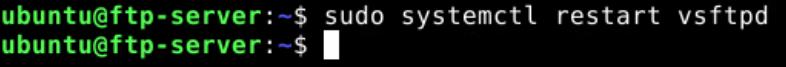
\includegraphics[width=\linewidth]{images/part2/step15.png}
    \end{center}

    \item Show the details of the \textbf{exercise-router} router. Take note of the IP address listed in the
    \textit{external\_gateway\_info} row.
\begin{lstlisting}
ubuntu@workstation:~$ openstack router show exercise-router
\end{lstlisting}

    \begin{center}
        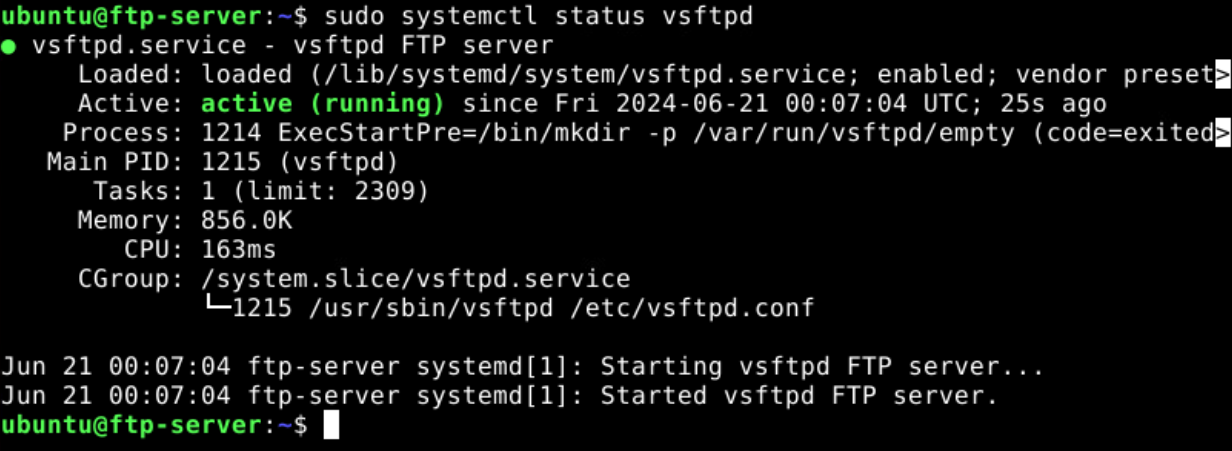
\includegraphics[width=\linewidth]{images/part2/step16.png}
    \end{center}

    \item SSH into the \textbf{devstack} virtual machine. Log in with the password \textbf{ubuntu}.
\begin{lstlisting}
ubuntu@workstation:~$ ssh 192.168.1.20
\end{lstlisting}

    \begin{center}
        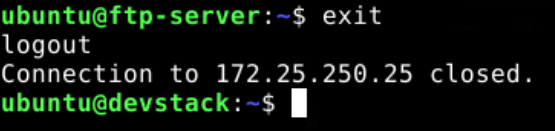
\includegraphics[width=\linewidth]{images/part2/step17.png}
    \end{center}

    \begin{tipbox}
        The password can be found on the EZSetup page showing the network topology for the lab. Click the
        \textbf{devstack} machine and click the eye icon under \textit{Password}.
    \end{tipbox}

    \item Use the \textbf{\texttt{ping}} command on the IP address found from the
    \textbf{\texttt{openstack router show}} command to verify that the router can be reached.
\begin{lstlisting}
ubuntu@devstack:~$ ping -c3 172.25.250.71
\end{lstlisting}

    \begin{notebox}{}
        The actual IP address may differ from this example.
    \end{notebox}

    \begin{center}
        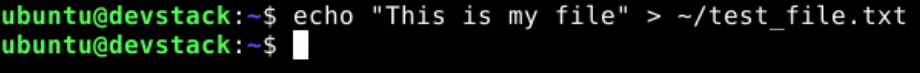
\includegraphics[width=\linewidth]{images/part2/step18.png}
    \end{center}

    \item Exit the SSH session.
\begin{lstlisting}
ubuntu@workstation:~$ exit
\end{lstlisting}

    \begin{center}
        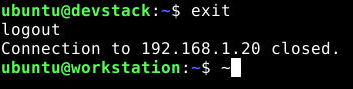
\includegraphics[width=\linewidth]{images/part2/step19.png}
    \end{center}

    \item Leave the terminal window open and continue to the next task.

\end{enumerate}

\section{Maintaining Floating IP Addresses}
\label{sec:maintaining_floating_ip_addresses}
In this task, you will create a set of floating IP addresses and allocate them to an instance.

\begin{enumerate}
    \item If a terminal window is not already open, open one and source the admin credentials from the 
    \textbf{\texttildemid/keystonerc-admin} file.

    \item Create a new instance named \textbf{instance1}. Use the \textbf{ubuntu} image, \textbf{m1.small} flavor, and
    \textbf{shared} network.
\begin{lstlisting}
ubuntu@workstation:~$ openstack server create \
> --image ubuntu \
> --flavor m1.small \
> --nic net-id=shared \
> --wait instance1
\end{lstlisting}

    \begin{center}
        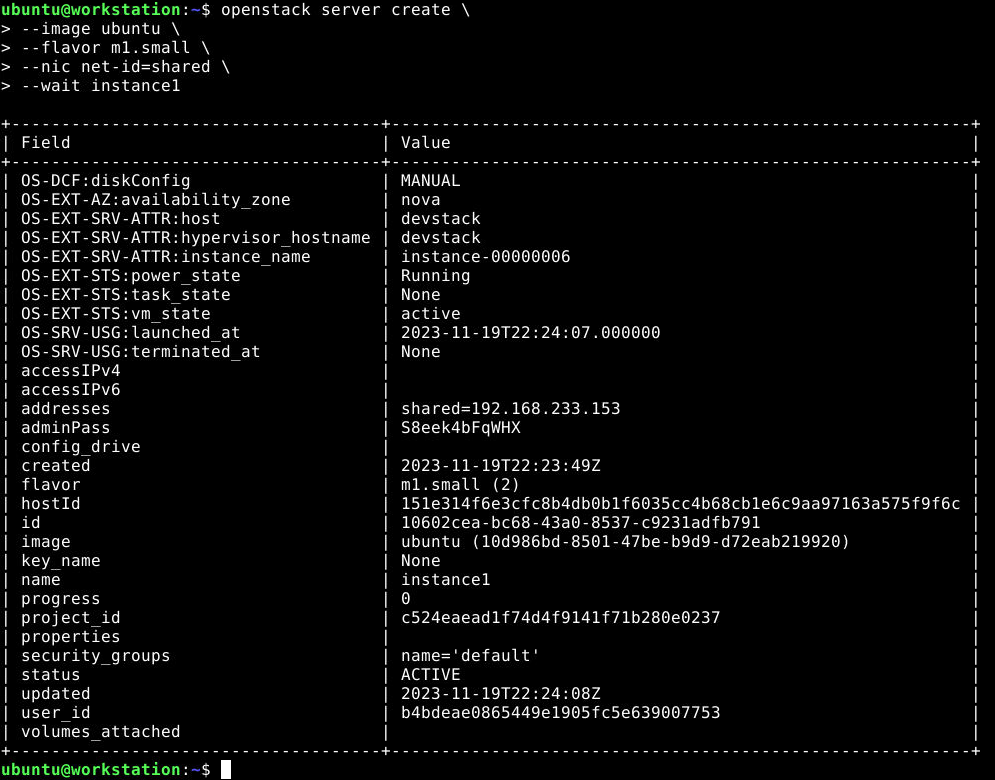
\includegraphics[width=\linewidth]{images/part3/step2.png}
    \end{center}

    \item Leave the terminal window open and open the web browser. Navigate to \textbf{192.168.1.20}. Log into the
    \textit{Horizon Dashboard} as the \textbf{admin} user with the password \textbf{secret}.


    \item Switch to the \textbf{demo} project. Navigate to \textbf{Project $>$ Network $>$ Floating IPs}. Click
    \textbf{Allocate IP to Project}.

    \begin{center}
        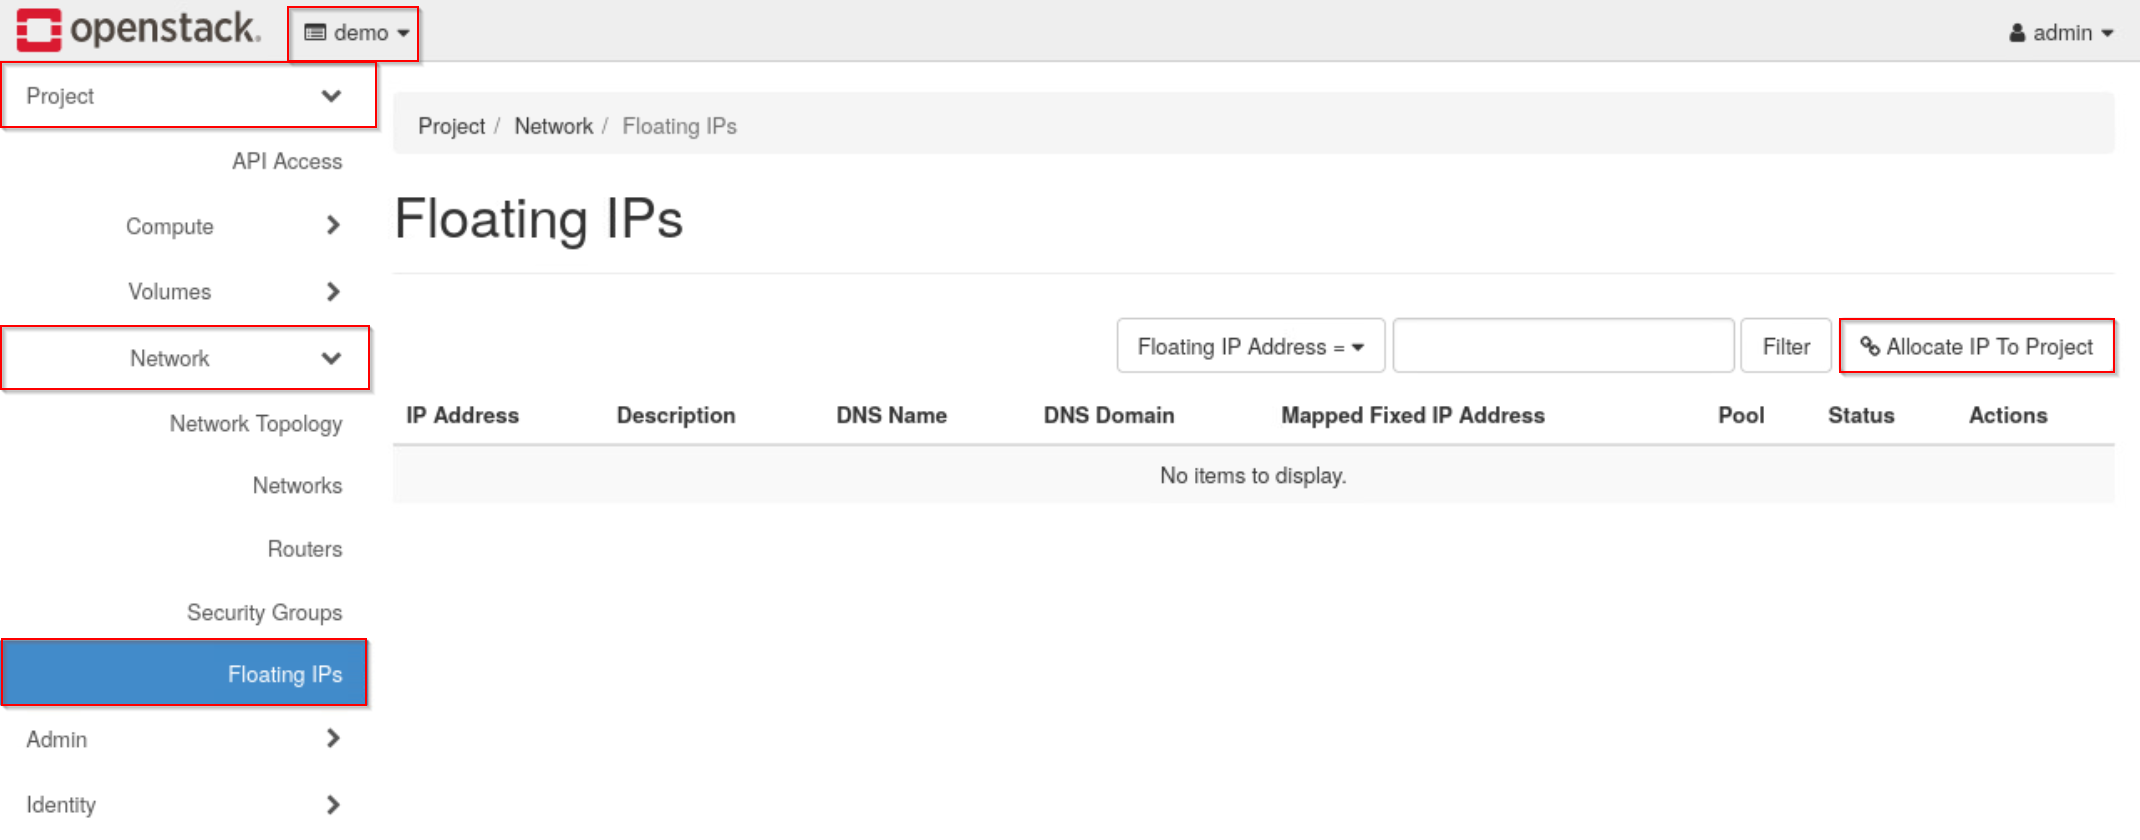
\includegraphics[width=\linewidth]{images/part3/step4.png}
    \end{center}

    \item Ensure \textbf{external} is set as the \textit{Pool}. Click \textbf{Allocate IP}.
    
    \begin{center}
        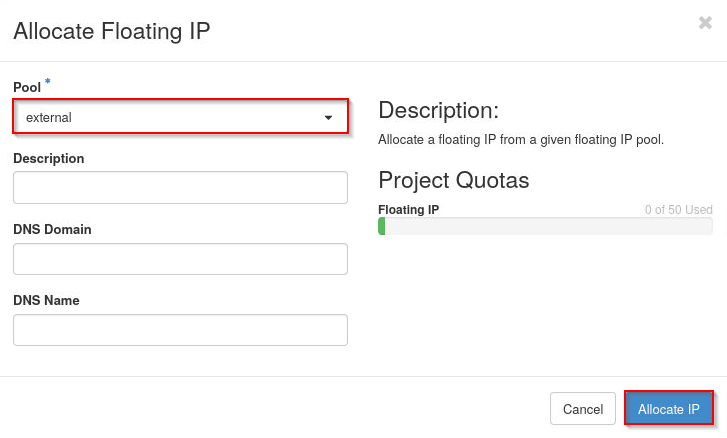
\includegraphics[width=\linewidth]{images/part3/step5.png}
    \end{center}

    \item Click \textbf{Associate} in the row of the floating IP address.

    \begin{center}
        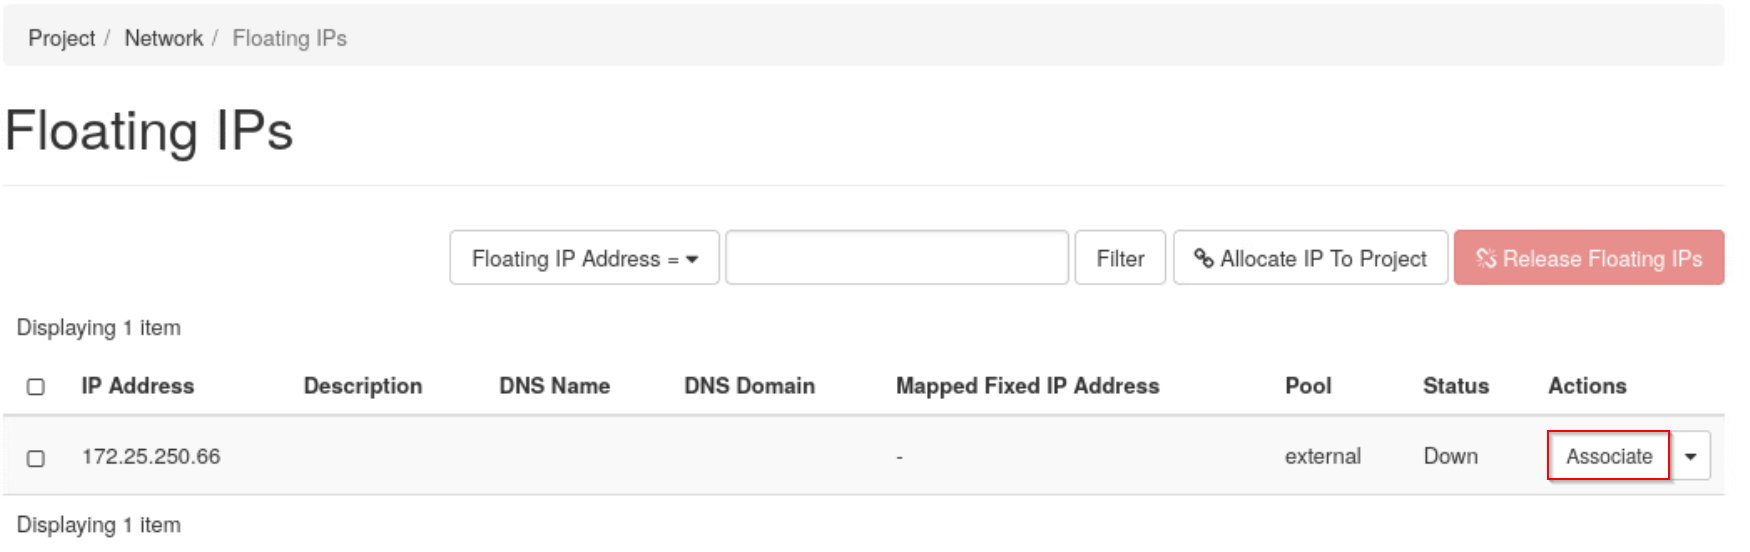
\includegraphics[width=\linewidth]{images/part3/step6.png}
    \end{center}
    
    \item In the \textit{Port to be associated} dropdown, select \textbf{instance1: 192.168.233.XYZ}. Click
    \textbf{Associate}.

    \begin{center}
        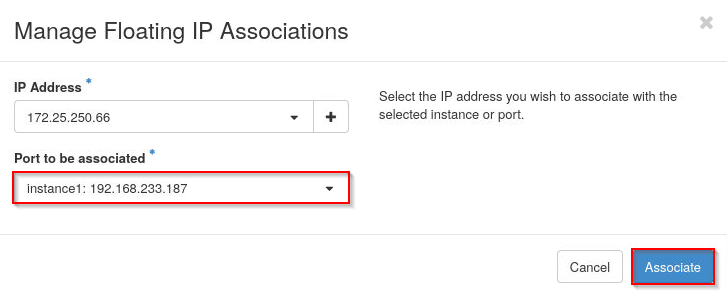
\includegraphics[width=\linewidth]{images/part3/step7.png}
    \end{center}

    \begin{notebox}{}
        The actual value of the floating IP address may differ.
    \end{notebox}

    \item Navigate to \textbf{Compute $>$ Instances}. Click the arrow next to the \textbf{Create Snapshot} in the same
    as \textbf{instance1}. Select \textbf{Disassociate Floating IP} to detach the floating IP from the instance.

    \begin{center}
        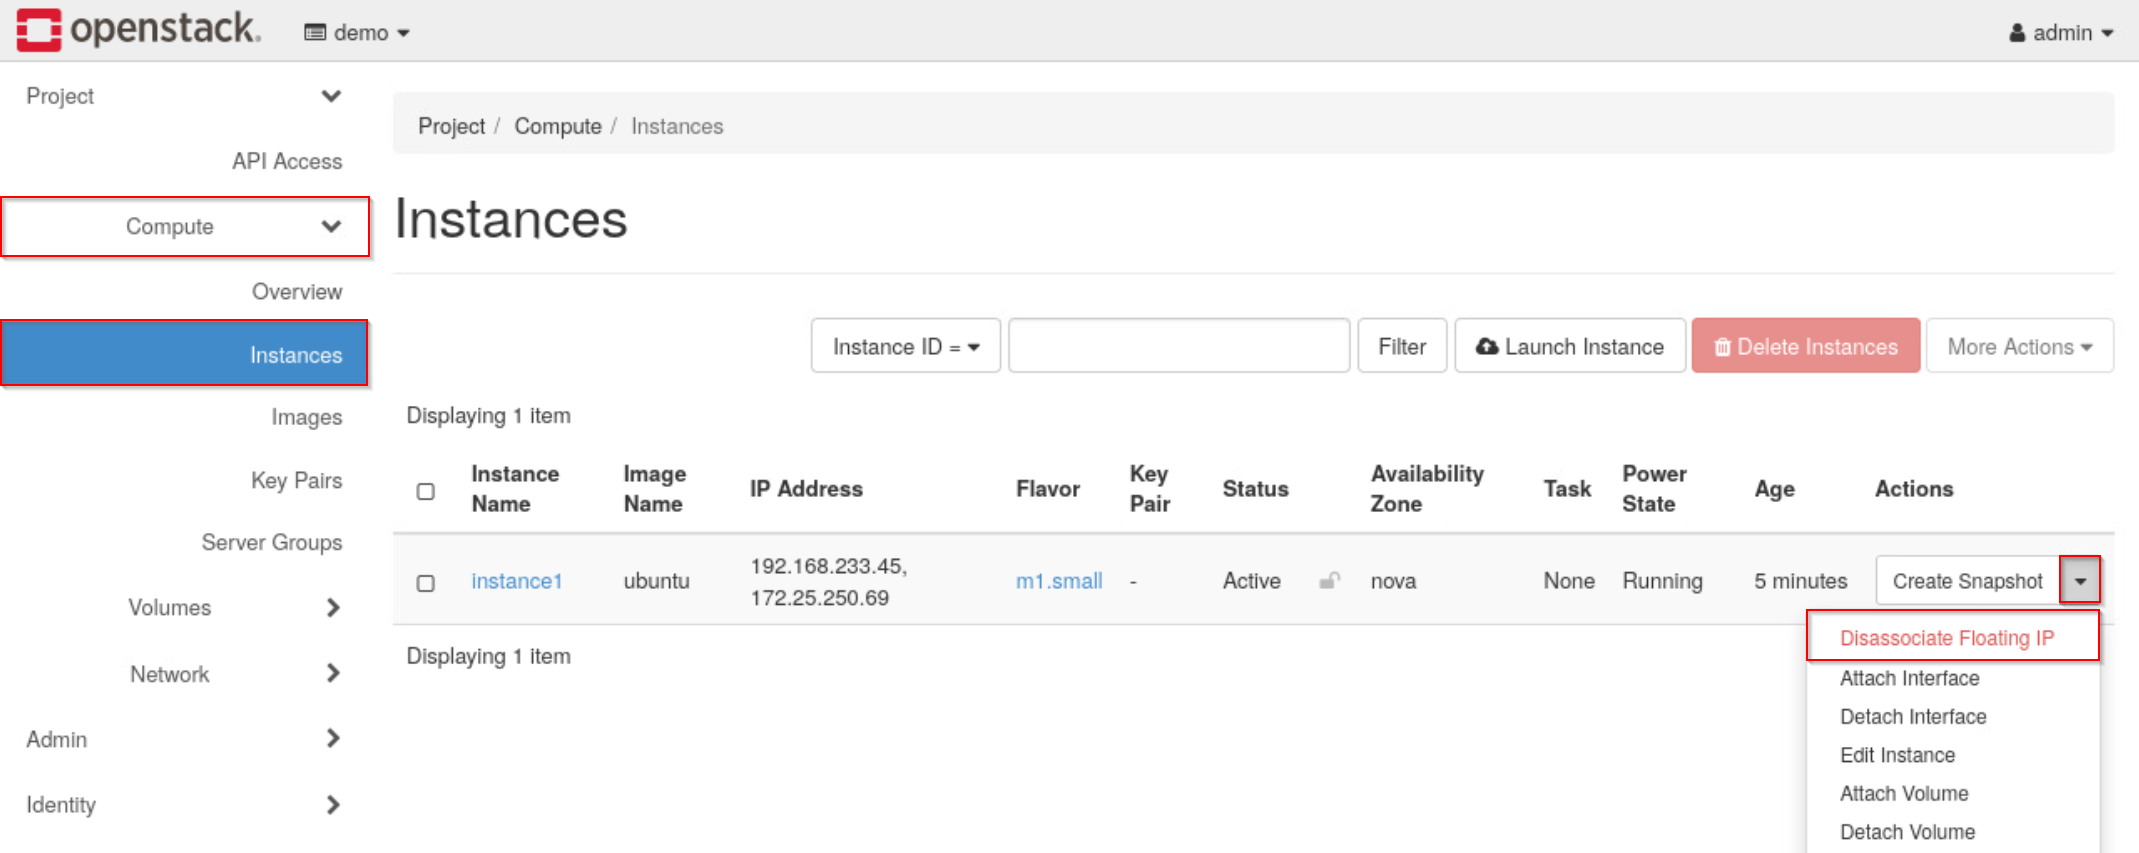
\includegraphics[width=\linewidth]{images/part3/step8.png}
    \end{center}

    \item Check the \textit{Release Floating IP} box and click \textbf{Disassociate}.
    
    \begin{center}
        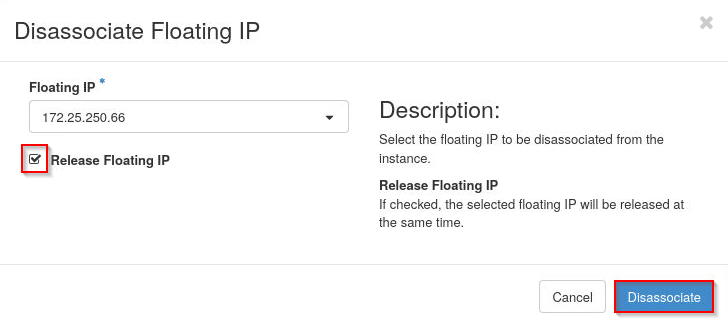
\includegraphics[width=\linewidth]{images/part3/step9.png}
    \end{center}

    \item Log out of the \textit{Horizon Dashboard} and close the web browser.

    \item From the terminal, create the floating IP \textbf{172.25.250.66} in the \textbf{external} network.
\begin{lstlisting}
ubuntu@workstation:~$ openstack floating ip create \
> --floating-ip-address 172.25.250.66 \
> external
\end{lstlisting}

    \begin{center}
        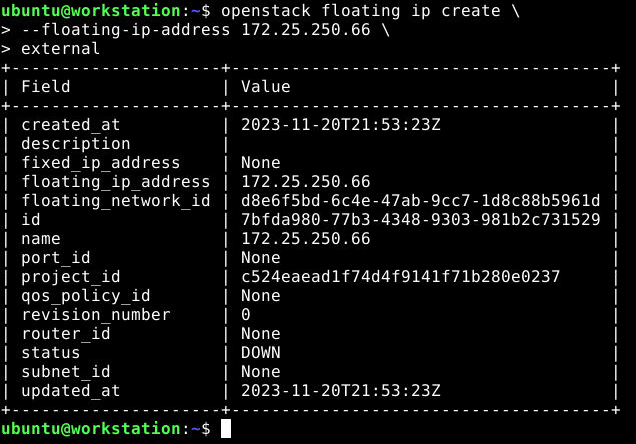
\includegraphics[width=\linewidth]{images/part3/step11.png}
    \end{center}

    \begin{tipbox}{}
        If an \textit{HttpException: Conflict} error appears, this indicates that a floating IP from a previous step in
        this section was not released. If this is the case, either go back to the \textit{Horizon Dashboard} and release
        the floating IP address or use the next available floating IP address.
    \end{tipbox}

    \item From the floating IP pool in the \textbf{external} network, create a floating IP.
\begin{lstlisting}
ubuntu@workstation:~$ openstack floating ip create external
\end{lstlisting}

    \begin{center}
        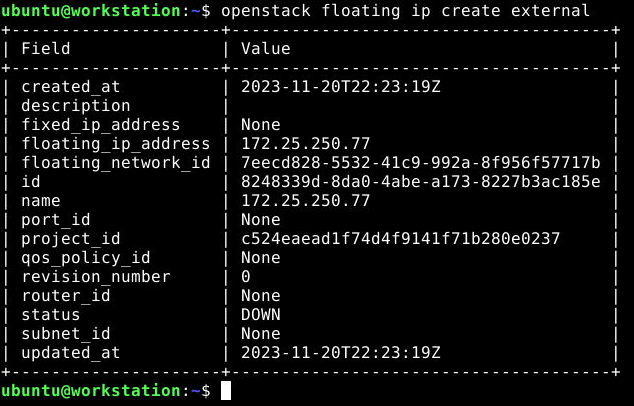
\includegraphics[width=\linewidth]{images/part3/step12.png}
    \end{center}

    \item Allocate a second floating IP using the same command.
\begin{lstlisting}
ubuntu@workstation:~$ openstack floating ip create external
\end{lstlisting}

    \begin{center}
        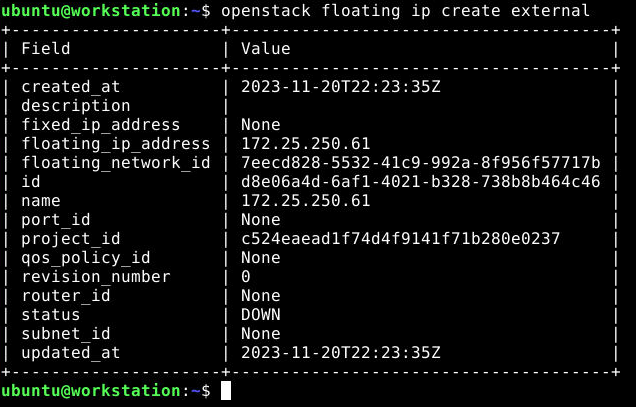
\includegraphics[width=\linewidth]{images/part3/step13.png}
    \end{center}

    \item Allocate a third floating IP.
\begin{lstlisting}
ubuntu@workstation:~$ openstack floating ip create external
\end{lstlisting}

    \begin{center}
        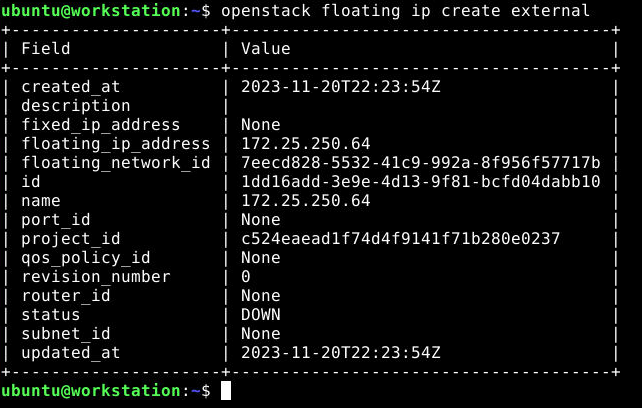
\includegraphics[width=\linewidth]{images/part3/step14.png}
    \end{center}

    \item Associate the third floating IP with \textbf{instance1}.
\begin{lstlisting}
ubuntu@workstation:~$ openstack server add \
> floating ip instance1 172.25.250.74
\end{lstlisting}

    \begin{center}
        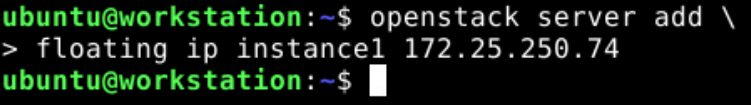
\includegraphics[width=\linewidth]{images/part3/step15.png}
    \end{center}

    \begin{notebox}{}
        The actual floating IP may differ. Use the floating IP address generated from your output from the previous
        step.
    \end{notebox}

    \item Leave the terminal window open and continue to the next task.

\end{enumerate}

\section{Implementing Security}
\label{sec:implementing_security}
In this task, you will use the \textit{Horizon Dashboard} and \textit{OpenStack Unified CLI} to manage SSH key pairs and
security groups for OpenStack instances.

\begin{enumerate}
    \item Open the web browser and navigate to \textbf{192.168.1.20}. Log into the dashboard as \textbf{admin} with the
    password \textbf{secret}.

    \item Switch to the \textbf{demo} project and navigate to \textbf{Project $>$ Compute $>$ Key Pairs}. Click
    \textbf{Create Key Pair} to create a new key pair.

    \begin{center}
        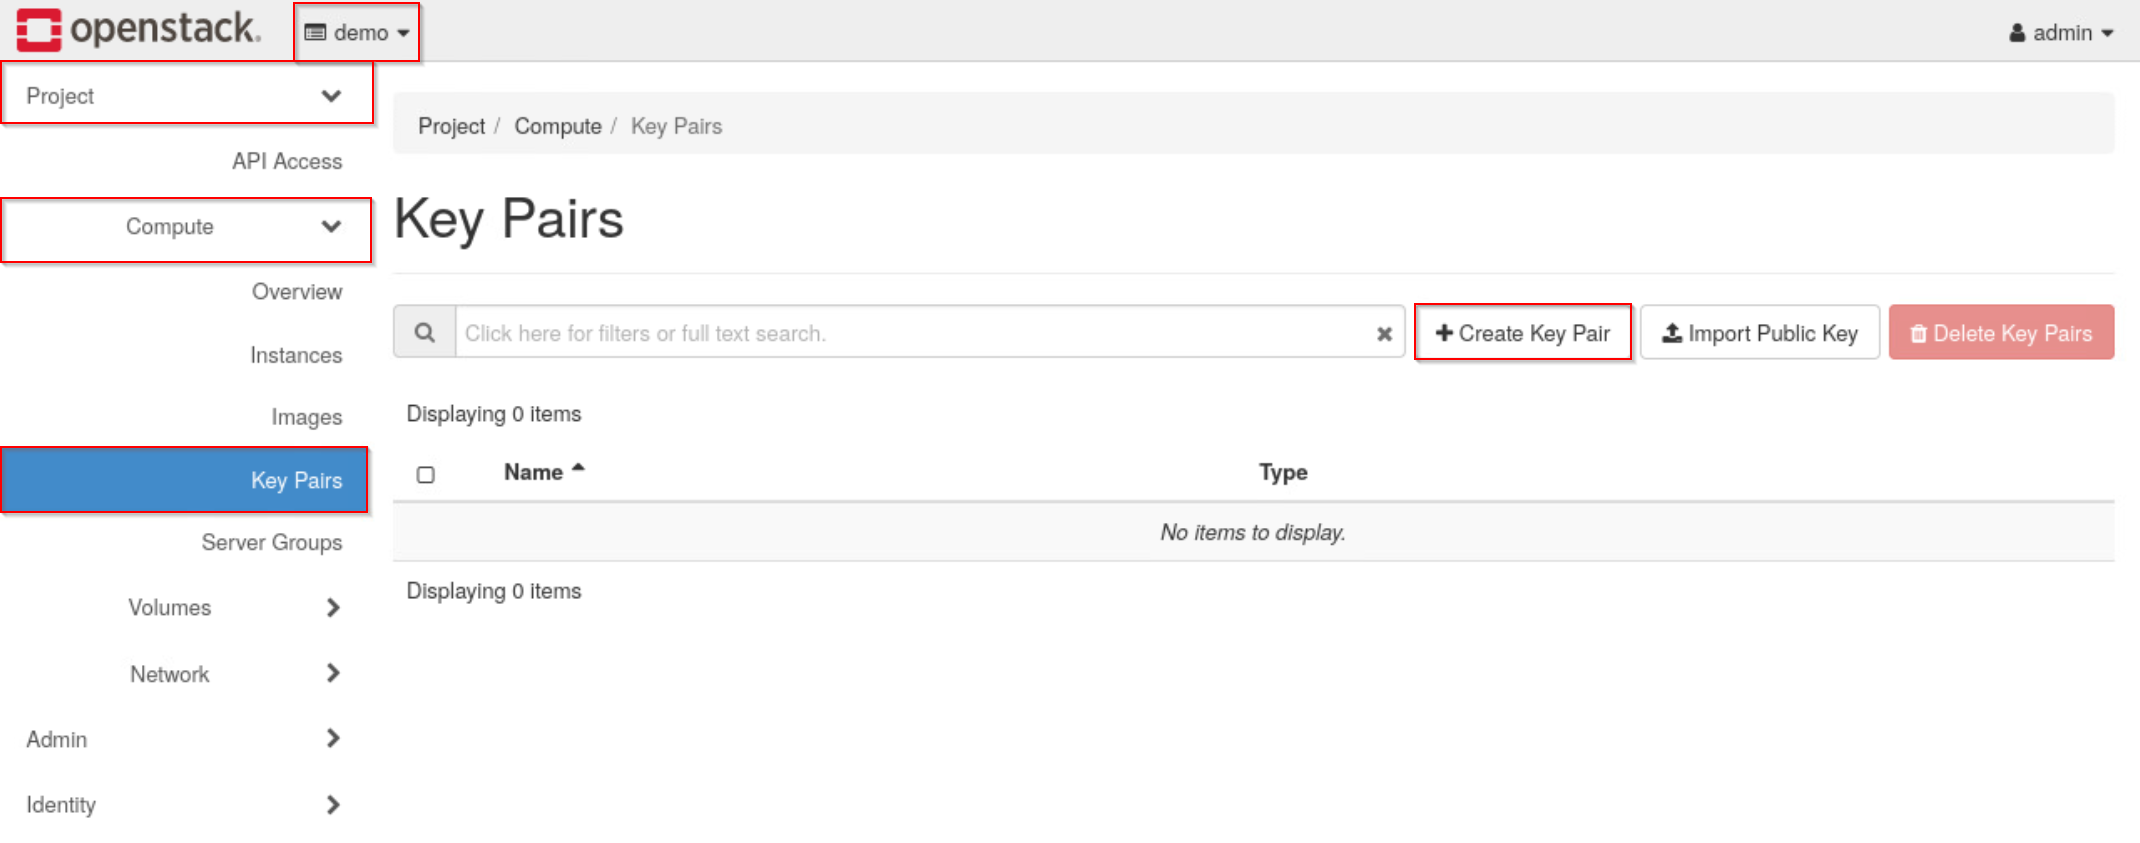
\includegraphics[width=\linewidth]{images/part4/step2.png}
    \end{center}

    \item Enter \textbf{keypair1} in the \textit{Key Pair Name} field, and select \textbf{SSH Key} in the \textit{Key
    Type} dropdown. Click \textbf{Create Key Pair}. This will create the key pair and download it to the
    \textbf{\texttildemid/Downloads} directory.

    \begin{center}
        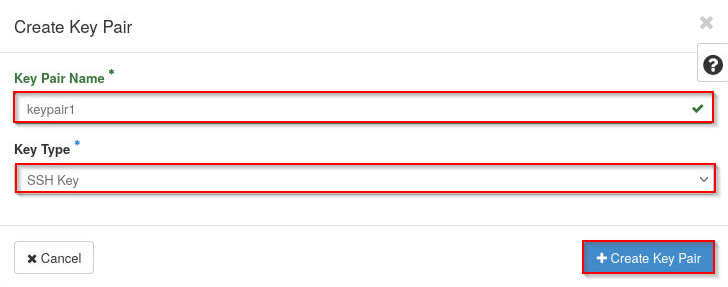
\includegraphics[width=\linewidth]{images/part4/step3.png}
    \end{center}

    \item Navigate to \textbf{Network $>$ Security Groups} and click \textbf{Create Security Group}.

    \begin{center}
        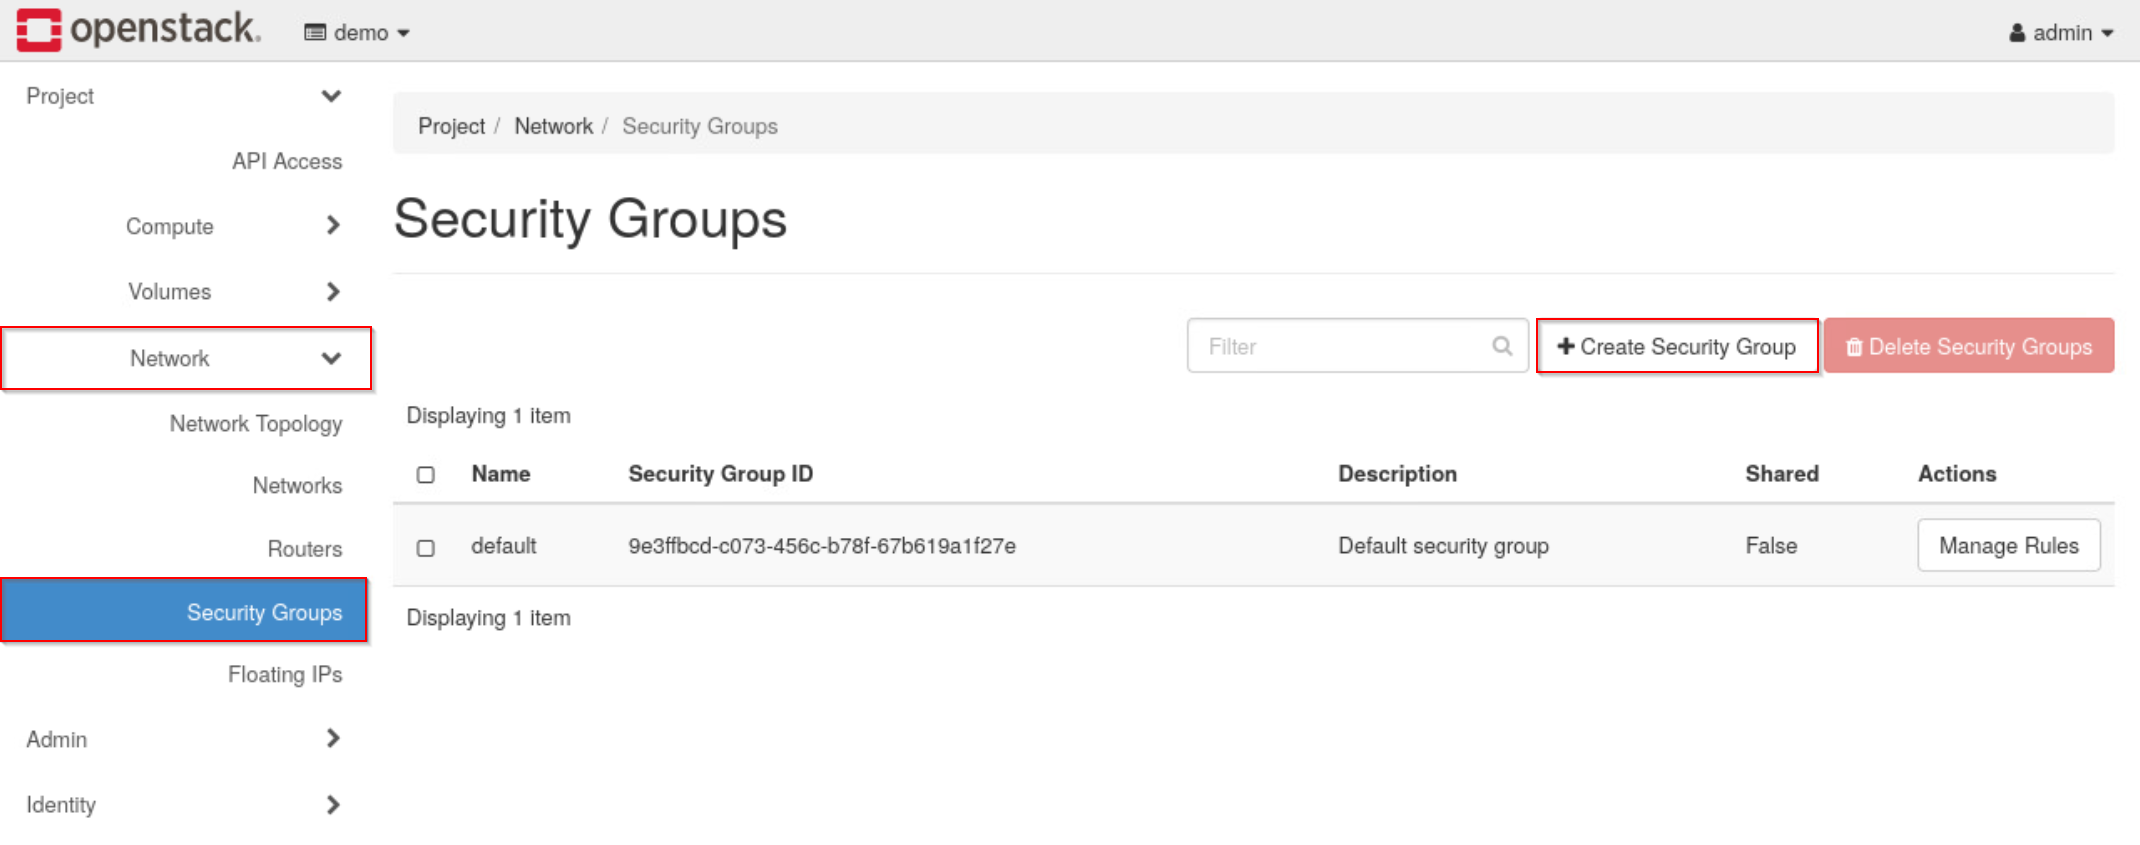
\includegraphics[width=\linewidth]{images/part4/step4.png}
    \end{center}

    \item Enter \textbf{secgroup1} into the \textit{Name} field and click \textbf{Create Security Group}.

    \begin{center}
        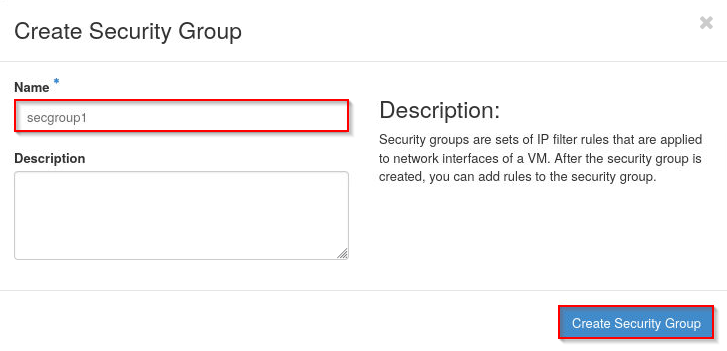
\includegraphics[width=\linewidth]{images/part4/step5.png}
    \end{center}

    \item After creating the security group, you should land on the page containing the rules for the security group.
    If not, click \textbf{Manage Rules} in the same column as \textbf{secgroup1} on the \textbf{Security Groups} page to
    get there. Click \textbf{Add Rule} to add a new rule in the security group.

    \begin{center}
        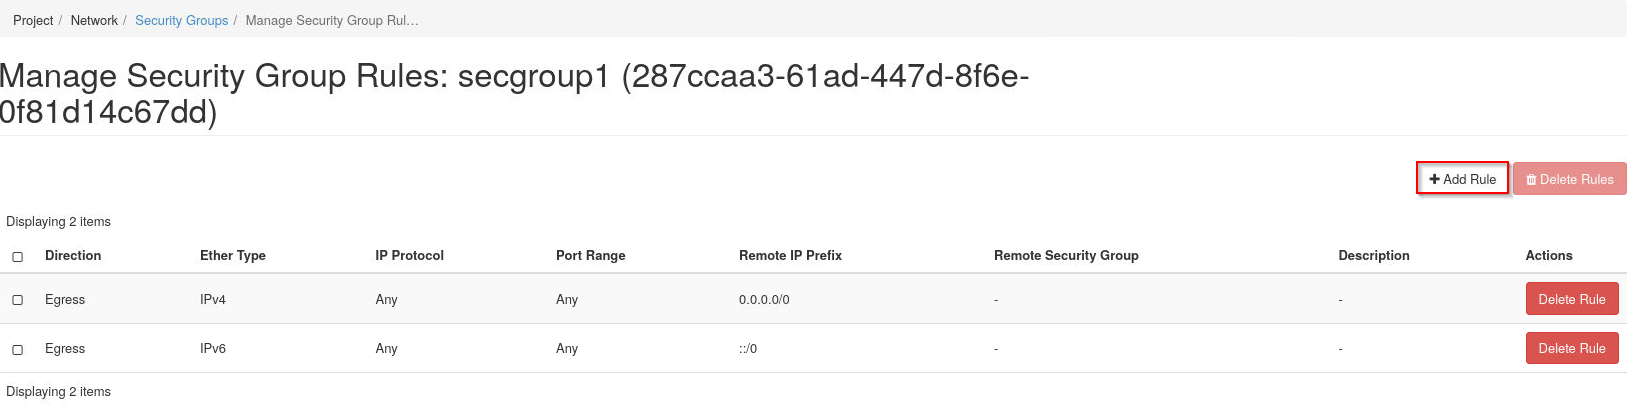
\includegraphics[width=\linewidth]{images/part4/step6.png}
    \end{center}

    \item Select \textbf{All ICMP} from the \textit{Rule} dropdown and click \textbf{Add}. This will allow ICMP traffic,
    namely the \textbf{\texttt{ping}} command, to reach instances in this security group.

    \begin{center}
        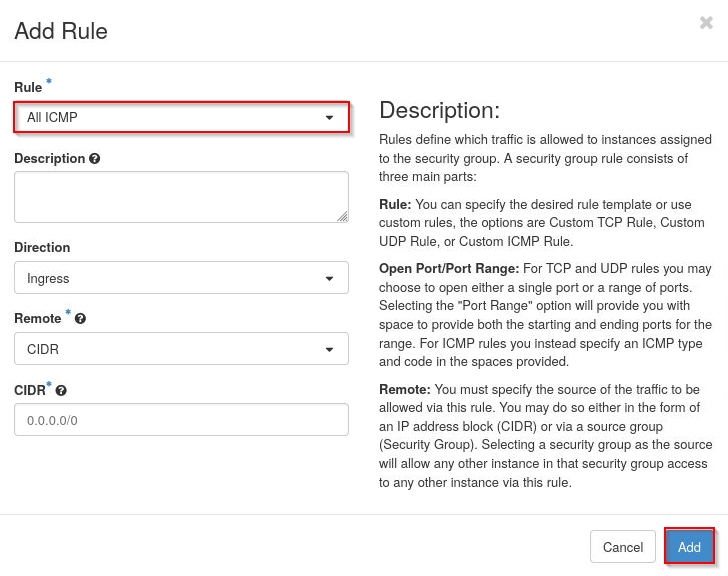
\includegraphics[width=\linewidth]{images/part4/step7.png}
    \end{center}

    \item Log out of the \textit{Horizon Dashboard} and close the web browser.
    
    \item If a terminal window is not already open, open one and source the \textbf{admin} credentials from the
    \textbf{\texttildemid/keystonerc-admin} file.

    \item Delete the private key located at \textbf{\texttildemid/Downloads/keypair1.pem}.
\begin{lstlisting}
ubuntu@workstation:~$ rm -f ~/Downloads/keypair1.pem
\end{lstlisting}

    \begin{center}
        \includegraphics[width=\linewidth]{images/part4/step10.png}
    \end{center}

    \item Delete the \textbf{keypair1} key pair.
\begin{lstlisting}
ubuntu@workstation:~$ openstack keypair delete keypair1
\end{lstlisting}

    \begin{center}
        \includegraphics[width=\linewidth]{images/part4/step11.png}
    \end{center}

    \item List the rules in the \textbf{secgroup1} security group.
\begin{lstlisting}
ubuntu@workstation:~$ openstack security group rule \
> list secgroup1
\end{lstlisting}

    \begin{center}
        \includegraphics[width=\linewidth]{images/part4/step12.png}
    \end{center}

    \item Use the \textit{ID} for the ICMP rule to delete that rule.
\begin{lstlisting}
ubuntu@workstation:~$ openstack security group rule \
> delete c92f0fdb-65b0-ae54-e9ec13ac98c1
\end{lstlisting}

    \begin{center}
        \includegraphics[width=\linewidth]{images/part4/step13.png}
    \end{center}

    \begin{notebox}{}
        The actual ID value may differ.
    \end{notebox}

    \item Delete the \textbf{secgroup1} security group.
\begin{lstlisting}
ubuntu@workstation:~$ openstack security group \
> delete secgroup1
\end{lstlisting}

    \begin{center}
        \includegraphics[width=\linewidth]{images/part4/step14.png}
    \end{center}

    \item Create the key pair \textbf{dev-keypair} and save the private key to the file
    \textbf{\texttildemid/Downloads/dev-keypair.pem}.
\begin{lstlisting}
ubuntu@workstation:~$ openstack keypair create \
> dev-keypair > ~/Downloads/dev-keypair.pem
\end{lstlisting}

    \begin{center}
        \includegraphics[width=\linewidth]{images/part4/step15.png}
    \end{center}

    \item the \textbf{\texttt{chmod}} command with a mode of \textbf{600} to make it so that the \textbf{ubuntu} user
    has read/write permissions on the file, and groups and other users have no permissions to the file.
\begin{lstlisting}
ubuntu@workstation:~$ chmod 600 ~/Downloads/dev-keypair.pem
\end{lstlisting}

    \begin{center}
        \includegraphics[width=\linewidth]{images/part4/step16.png}
    \end{center}

    \item Create the \textbf{dev-secgroup} security group.
\begin{lstlisting}
ubuntu@workstation:~$ openstack security group \
> create dev-secgroup
\end{lstlisting}

    \begin{center}
        \includegraphics[width=\linewidth]{images/part4/step17.png}
    \end{center}

    \item Add a security rule in the \textbf{dev-secgroup} security group to allow remote ICMP traffic.
\begin{lstlisting}
ubuntu@workstation: openstack security group \
> rule create \
> --protocol icmp \
> dev-secgroup
\end{lstlisting}

    \begin{center}
        \includegraphics[width=\linewidth]{images/part4/step18.png}
    \end{center}

    \item Add another security rule to allow remote connection using SSH on the default port 22.
\begin{lstlisting}
ubuntu@workstation:~$ openstack security group \
> rule create \
> --protocol tcp \
> --dst-port 22 \
> dev-secgroup
\end{lstlisting}

    \begin{center}
        \includegraphics[width=\linewidth]{images/part4/step19.png}
    \end{center}

    \item Open the web browser and navigate to \textbf{192.168.1.20}. Log into the dashboard as \textbf{admin} with the
    password \textbf{secret}.

    \item Navigate to \textbf{Project $>$ Floating IPs}. Disassociate the floating IP assigned to \textbf{instance1}.

    \begin{center}
        \includegraphics[width=\linewidth]{images/part4/step21.png}
    \end{center}

    \item Click \textbf{Disassociate} to confirm the disassociation.
    
    \begin{center}
        \includegraphics[width=\linewidth]{images/part4/step22.png}
    \end{center}

    \item Select all checkboxes and click \textbf{Release Floating IPs} to release all the floating IP addresses.
    
    \begin{center}
        \includegraphics[width=\linewidth]{images/part4/step23.png}
    \end{center}

    \item Click \textbf{Release FLoating IPs} to confirm the release of the all the floating IP addresses.
    
    \begin{center}
        \includegraphics[width=\linewidth]{images/part4/step24.png}
    \end{center}

    \item Navigate to the \textbf{Routers} tab. Click the \textbf{Clear Gateway} associated with
    \textbf{exercise-router} to remove its interface on the \textbf{external} network.

    \begin{center}
        \includegraphics[width=\linewidth]{images/part4/step25.png}
    \end{center}
    
    \item Click \textbf{Clear Gateway} to confirm the clearing of the gateway.
    
    \begin{center}
        \includegraphics[width=\linewidth]{images/part4/step26.png}
    \end{center}

    \item Navigate to \textbf{Compute $>$ Instances}. In the row for the \textbf{instance1} instance, click the
    dropdown next to the \textbf{Create Snapshot} button, then click \textbf{Detach Interface}.

    \begin{center}
        \includegraphics[width=\linewidth]{images/part4/step27.png}
    \end{center}

    \item In the \textbf{Detach Interface} window, select \textbf{192.168.233.XYZ} and click \textbf{Detach Interface}.
    
    \begin{center}
        \includegraphics[width=\linewidth]{images/part4/step28.png}
    \end{center}

    \item Click the checkbox next to \textbf{instance1}, then click \textbf{Delete Instances}.
    
    \begin{center}
        \includegraphics[width=\linewidth]{images/part4/step29.png}
    \end{center}

    \item Click \textbf{Delete Instances} to confirm the deletion of \textbf{instance1}.
    
    \begin{center}
        \includegraphics[width=\linewidth]{images/part4/step30.png}
    \end{center}

    \item Close the web browser and continue to the next task.

\end{enumerate}

\section{Launching an External Instance}
\label{sec:launching_an_external_isntance}
In this task, you will launch an external instance.

\begin{enumerate}
    \item If a terminal window is not already open, open one and source the admin credentials from the 
    \textbf{\texttildemid/keystonerc-admin} file.

    \item List all instances in the project. The list should be empty.
\begin{lstlisting}
ubuntu@workstation:~$ openstack server list
\end{lstlisting}

    \begin{center}
        \includegraphics[width=\linewidth]{images/part5/step2.png}
    \end{center}

    \item Launch an instance named \textbf{instance-external} using the \textbf{ubuntu} image, the \textbf{m1.small}
    flavor, the \textbf{dev-keypair} key pair, the \textbf{shared} network, and the \textbf{dev-secgroup} security
    group.
\begin{lstlisting}
ubuntu@workstation:~$ openstack server create \
> --image ubuntu \
> --flavor m1.small \
> --key-name dev-keypair \
> --nic net-id=shared \
> --security-group dev-secgroup \
> --wait instance-external
\end{lstlisting}

    \begin{center}
        \includegraphics[width=\linewidth]{images/part5/step3.png}
    \end{center}

    \item Set the \textbf{external} network as the gateway for the \textbf{exercise-router} router.
\begin{lstlisting}
ubuntu@workstation:~$ openstack router set \
> --external-gateway external \
> exercise-router
\end{lstlisting}

    \begin{center}
        \includegraphics[width=\linewidth]{images/part5/step4.png}
    \end{center}

    \item Create a floating IP address for the project.
\begin{lstlisting}
ubuntu@workstation:~$ openstack floating ip create external
\end{lstlisting}

    \begin{center}
        \includegraphics[width=\linewidth]{images/part5/step5.png}
    \end{center}

    \item Create a second floating IP address for the project.
\begin{lstlisting}
ubuntu@workstation:~$ openstack floating ip create external
\end{lstlisting}

    \begin{center}
        \includegraphics[width=\linewidth]{images/part5/step6.png}
    \end{center}

    \item Create a third floating IP address for the project.
\begin{lstlisting}
ubuntu@workstation:~$ openstack floating ip create external
\end{lstlisting}

    \begin{center}
        \includegraphics[width=\linewidth]{images/part5/step7.png}
    \end{center}

    \item Associate the third floating IP address with the \textbf{instance-external} instance.
\begin{lstlisting}
ubuntu@workstation;~$ openstack server add floating ip \
> instance-external 172.25.250.74
\end{lstlisting}

    \begin{center}
        \includegraphics[width=\linewidth]{images/part5/step8.png}
    \end{center}

    \begin{notebox}{}
        Be sure to use the floating IP address that matches your output as they may differ slightly from this example.
    \end{notebox}

    \item Verify that the instance was assigned the floating IP address.
\begin{lstlisting}
ubuntu@workstation:~$ openstack server list \
> -c Name \
> -c Networks
\end{lstlisting}

    \begin{center}
        \includegraphics[width=\linewidth]{images/part5/step9.png}
    \end{center}

    \begin{tipbox}{}
        For commands that output tables, you can pull out only the columns you want by using the \textbf{\texttt{-c}}
        option followed by the column name. This option can be chained as in the command above to list multiple columns.
    \end{tipbox}

    \item Leave the terminal window open and continue to the next task.
\end{enumerate}

\section{Verifying an External Instance}
\label{sec:verifying_an_external_instance}
In this task, you will verify the functionality of an external instance by using the \textbf{\texttt{ssh}} and
\textbf{\texttt{ping}} commands to test the external network.

\begin{enumerate}
    \item If a terminal window is not already open, open one and source the admin credentials from the 
    \textbf{\texttildemid/keystonerc-admin} file.

    \item Use the \textbf{\texttt{scp}} command to send the \textbf{dev-keypair} key pair to the \textbf{devstack}
    machine over the SSH protocol.
\begin{lstlisting}
ubuntu@workstation:~$ scp ~/Downloads/dev-keypair.pem \
> ubuntu@192.168.1.20:~/dev-keypair.pem
\end{lstlisting}

    \begin{center}
        \includegraphics[width=\linewidth]{images/part6/step2.png}
    \end{center}

    \item SSH into the \textbf{devstack} machine.
\begin{lstlisting}
ubuntu@workstation:~$ ssh 192.168.1.20
\end{lstlisting}

    \begin{center}
        \includegraphics[width=\linewidth]{images/part6/step3.png}
    \end{center}

    \item Ping the \textbf{external-instance} instance using the floating IP that was assigned to it in the previous
    task.
\begin{lstlisting}
ubuntu@devstack:~$ ping -c3 172.25.250.74
\end{lstlisting}

    \begin{center}
        \includegraphics[width=\linewidth]{images/part6/step4.png}
    \end{center}

    \item SSH into the \textbf{instance-external} instance, using the \textbf{dev-keypair.pem} file to authenticate.

    \begin{center}
        \includegraphics[width=\linewidth]{images/part6/step5.png}
    \end{center}

    \item Ping the DHCP server.
\begin{lstlisting}
ubuntu@instance-external:~$ ping -c3 192.168.233.2
\end{lstlisting}

    \begin{center}
        \includegraphics[width=\linewidth]{images/part6/step6.png}
    \end{center}

    \item The lab is now complete.

\end{enumerate}

\end{document}